\chapter{Crowdsourcing strategies in Pl@ntNet citizen based learning platform}
\label{chap:plantnet}
\enlargethispage{3\baselineskip}

\begin{keypointstwomargins}{Pl@ntNet}{-2cm}{-1cm}
        \textbf{Key points -- Crowdsourcing plant species}
        \begin{enumerate}[leftmargin=*]
        \item Aiding botanists in plant species identification is a challenging task. Species are often visually close and their identification requires expert knowledge.
        \item Pl@ntNet is a citizen science platform that allows users to upload images of plants and receive a list of possible species.
        \item The collaborative aspect of Pl@ntNet allows users to vote on the species they think are present in the image and contribute to new labeled data, which is then used to train a computer vision and help new identifications.
        \end{enumerate}

        \textbf{Contributions -- Exploration of Pl@ntNet label aggregation strategy}
        \begin{enumerate}[leftmargin=*,start=4]
        \item We release and evaluate the current Pl@ntNet label aggregation and compare it to other strategies.
        \item We release a subset of Pl@ntNet with images url and collected labels in the South Western European Flora of more than $6$ million observations and $800$ thousand users in a large-scale classification setting.
        \item We discuss how to integrate the current model's predictions in the votes aggregation. This is a challenging task due to the iterative aspect of Pl@ntNet: the current data helps train the next generation of models iteratively.
        \end{enumerate}
\end{keypointstwomargins}

While crowdsourcing is advertised to collect a large number of data easily, with strategies to mitigate the noise, openly available datasets are still scarce and with a low number of classes ($K\leq 10$ in general).
In this chapter, we focus on the Pl@ntNet platform, a citizen science platform for plant species recognition.
One of the challenges in this classification setting is the large number of possible species ($K>10^4$).
After presenting the platform and voting system, we will investigate the current label aggregation strategy in Pl@ntNet.
We compare it with other strategies that can handle this large number of classes, workers and tasks.
Finally, we propose to improve the current algorithm by taking advantage of the Pl@ntNet pipeline.

Note that in previous chapters, the crowdsourcing experiments concerned workers paid to answer multiple tasks.
In Pl@ntNet, contributions are by volunteers and the tasks are not paid.
We thus slightly adapt the vocabulary used in this chapter to reflect this difference.
People voting are called users.
The tasks are observations of plants (detailed in \Cref{sub:obs_plantnet_what}) for which we wish to identify the species.
% To reflect this change, we write $\mathcal{U}$ the set of all users. Each user $u$ has a unique identifier used as an index, and we denote $\mathcal{U}_i$ the set of users that have voted on observation $i$.
% We thus have $\mathcal{U} = \bigcup_{i\in [n_\texttt{task}]} \mathcal{U}_i$.
% The vote of user $u$ on observation $i$ is denoted $y_i^{(j)}\in [K]$.

\section{Crowdsourcing for plant species identification}
\label{sec:introducing_plantnet}

Computer vision models are a great aid in plant species recognition in the field \citep{vidal2021perspectives,borowiec2022,mader2021flora}.
However, to train them one needs large annotated datasets.
These datasets are usually created thanks to crowdsourcing, but citizen science approaches, collecting both reliable and useful information \citep{brown2019potential,wright2021pixelwise}, tend to be more and more popular.
Among existing plant recognition applications, the Pl@ntNet citizen science platform \citep{affouard2017pl} enables global data collection by allowing users to upload and annotate plant observations \citep{bonnet2020citizen}.

We first introduce the problem of labeling a plant observation and the complexity of plant taxonomy.
Then, we present the Pl@ntNet platform and its voting interface.
Finally, we discuss the current label aggregation strategy and propose ways to improve it.

\subsection{Plant taxonomy generalities}
First, we need to understand the complexity of plant taxonomy.
Our goal here is to briefly present this taxonomy.
Plants are divided following a hierarchy, from the most general to the most specific ranks of taxa: kingdom, division, class, order, family, genus, and species according to the International Code of Nomenclature for algae, fungi, and plants (ICN) \citep{turland2018international}.
Each of these units of biological classification is called a taxon (taxa in plural).
Further secondary ranks also exist (tribe, subspecies, variety, form) but we will focus on the main ones.

Roughly, an example of taxonomy levels is:
\begin{itemize}
        \item Kingdom: separates plants from animals, fungi, and bacteria -- \emph{e.g} Plantae.
        \item Division: separates spore (\emph{angiosperms}) or seed (\emph{gymnosperms}) reproduction with specific characteristics. There are 14 plant divisions in total.
        \item Class: Angiosperms are divided into Monocotyledons(grasses, yuccas, etc.) and Dicotyledons (angiosperms with pair of leaves).
        \item Order: Group of families with common characteristics -- \emph{e.g} \emph{Cucurbitales} (generally ends with \emph{-ales}).
        \item Family: Plants with similar flower, fruit and seed structures -- \emph{e.g} \emph{Begonaias and Allies}.
        \item Genus (genera in plural): First part of the plant's scientific name (capitalized and italicized) -- \emph{e.g} \emph{Begonia}.
        \item Species: a group of organisms capable of producing fertile offspring -- \emph{e.g} \emph{Begonia ferox}. If the species is unknown it is called \emph{sp.} or \emph{spp.} for plural.
    \end{itemize}

\begin{figure}[htbp]
    \centering
    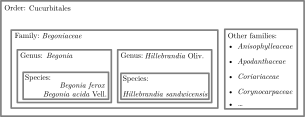
\includegraphics[width=.7\textwidth]{./images_plantnet/categories_begonia.pdf}
    \caption{\emph{Begonia ferox}: a species from the \emph{Begonia} genus of the \emph{Begoniaceae} family of the Cucurbitales order.}
    \label{fig:classif_begonia}
\end{figure}

In the case a plant is a hybrid -- a cross between two species -- it is written with an × as in \emph{Begonia} × \emph{semperflorens}. The position of the × indicates if it is the hybridization between two genera or species.
For example, the ×\emph{Agroelymus hajastanica} is the hybridization of the \emph{Agropyron cristatum} and the \emph{Elymus repens} -- note that the genera are aggregating into a resulting genus.
Similarly to the ×, a + is used to indicate a transplant chimera between two plants.
For example, the + \emph{Laburnocytisus adamii} results of the transplant of two individuals with different genera: the \emph{Laburnum anagyroides} and the \emph{Cytisus purpureus}.


\subsubsection{Checklists and referentials}

The plant name is generally composed of only two parts: the genus and the species.
In this work, we do not consider vernacular names -- the common names of plants -- as they can vary from one region to another.
Botanists have created checklists of accepted plant species.

One of the largest is the International Plant Names Index (IPNI) \citep{IPNI2024}.
The IPNI is a database of the published names and indicates which names are validly published.
It does not take into account the taxonomic status of the names -- the chronological changes and synonymity.
The World Checklist of Vascular Plants (WCVP) \citep{govaerts2021world} is an international collaborative database of taxa that provides the latest nomenclatural and taxonomic information on vascular plants -- \emph{clubmosses}, \emph{horsetails}, \emph{ferns}, \emph{gymnosperms} (including conifers), and \emph{angiosperms} (flowering plants).
The data from WCVP is the backbone for Plants Of the World Online (POWO)\footnote{\url{https://powo.science.kew.org}} which is an interface to access more information on individual species as their distribution for example.

There are multiple other checklists and databases such as The Plant List (TPL) \citep{PlantList2013}, the Catalogue of Life (CoL) \citep{cachuela2006towards}, Leipzig Catalogue of Vascular Plants (LCVP) \citep{freiberg2020leipzig} \emph{etc.} For a more exhaustive comparison of these databases we refer the reader to \citet{schellenberger2023big}.
The Global Biodiversity Information Facility (GBIF) \citep{telenius2011biodiversity} is an openly accessible network of shared knowledge about biodiversity on Earth.
They currently regroup $105$ different sources of taxonomy\footnote{\url{https://www.gbif.org/fr/dataset/d7dddbf4-2cf0-4f39-9b2a-bb099caae36c}}.

These checklists are the backbone of any botanical project as they provide a reference for the species names, their taxonomic status, and synonymic contributions.
Synonyms are not rare in plant taxonomy and can be due to different reasons such as the same species being described by different botanists, at different times, in different regions of the world.
As an example, in WCVP there are $\num{357347}$ plant species and $\num{565200}$ synonyms for those species.

Moreover, note that checklists might not always cover all the species and synonyms from one another.
For example, the \emph{Pilosella officinarum} Vaill. is listed in POWO with $161$ possible synonyms  -- $141$ accepted synonyms and $20$ illegitimate -- while in the GBIF it is listed with $241$ possible synonyms.
In the Pl@ntNet database, synonyms are only considered at the species level, resulting in $22$ possible accepted synonyms for this species.

\begin{figure}[tbh]
        \centering
        \includegraphics[width=.95\textwidth]{./images_plantnet/level2.pdf}
        \caption{Regional areas at level 2: subcontinental botanical regions of the world.  }
        \label{fig:level2}
\end{figure}

The international system groups areas of the world at different levels to record plant distributions and have standardized comparisons. This system is called the World Geographical Scheme for Recording Plant Distributions (WGSRPD) \citep{brummitt2001world}. The first level represents the nine botanical continents -- Europe, Africa, Asia-Temperate, Asia-Tropica, Australasia, Pacific, Northern America, Southern America and Antarctic.
The second level is the subcontinental regions of the world -- see \Cref{fig:level2} for a representation. It divides each botanical continent between $2$ and $10$ subdivisions. For example, Europe is divided into Northern, Middle, Southwestern, Southeastern and Eastern Europe.
Levels 3 and 4 include states, provinces or botanical areas.
In Pl@ntNet, level 2 is used to filter the species that can be observed in a given area and adapt the models' predictions.
In addition, users can specify to which flora -- either a level 2 subdivision or a Pl@ntNet project like "Useful plants" or "World Flora" -- they wish to associate their contribution.

\subsection{What is a plant observation?}
\label{sub:obs_plantnet_what}

\begin{figure}[bth]
        \centering
        \begin{minipage}[b]{0.3\textwidth}
            \centering
            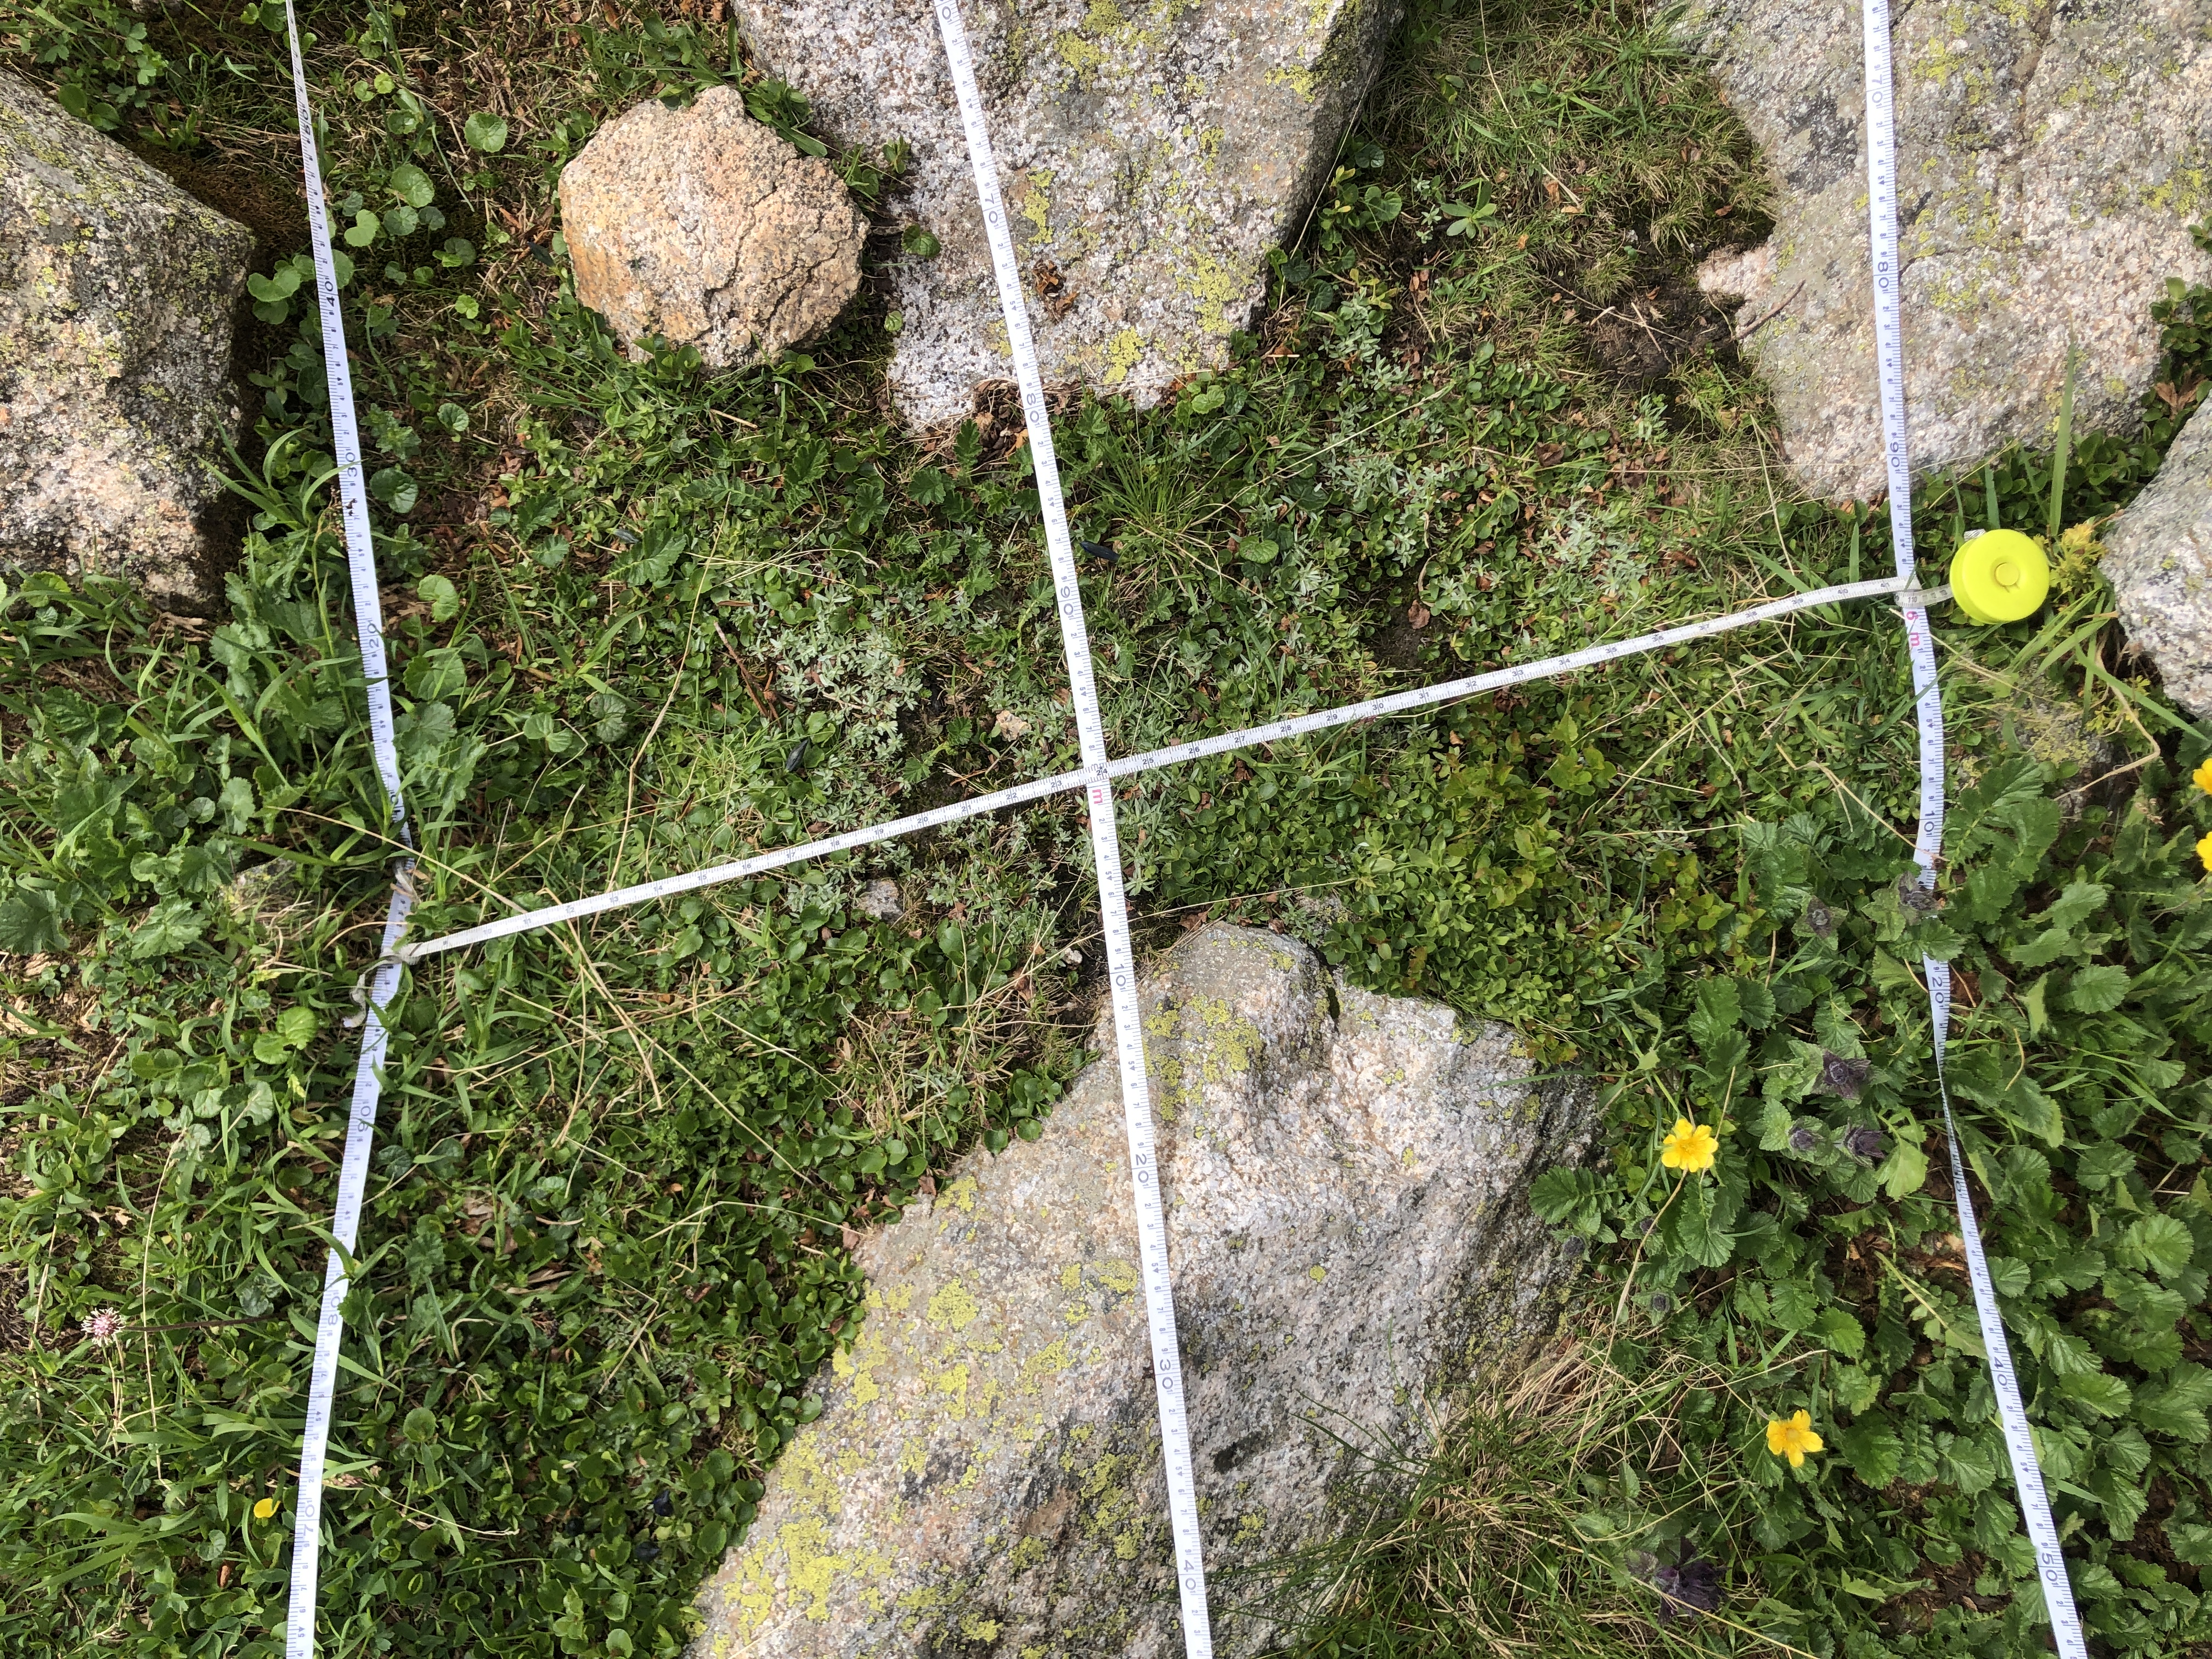
\includegraphics[width=\textwidth,height=4cm]{./images_plantnet/quadra1.JPG}
        %     \caption{Caption for Image 1}
        %     \label{fig:image1}
        \end{minipage}
        \hfill
        \begin{minipage}[b]{0.3\textwidth}
            \centering
            \includegraphics[width=\textwidth,height=4cm]{/images_plantnet/quadra2.jpeg}
        %     \caption{Caption for Image 2}
        %     \label{fig:image2}
        \end{minipage}
        \hfill
        \begin{minipage}[b]{0.3\textwidth}
            \centering
            \includegraphics[width=\textwidth,height=4cm]{./images_plantnet/quadra3.jpeg}
        %     \caption{Caption for Image 3}
        %     \label{fig:image3}
        \end{minipage}
        \caption{Quadrats used in the field to estimate the abundance of species. They are often in a hard rectangle shape material like wood or soft with meters of ribbon to delimit the surface. (\textcopyright Pierre Bonnet)}
        \label{fig:quadrats}
    \end{figure}

Contrary to classical datasets, Pl@ntNet observations are not a single image but a set of images taken by a user in the field.
A single image of a plant might not be enough to identify the species.
More images of different parts of the plant -- leaves, flowers, fruits, \emph{etc.} -- are needed to correctly identify the species and mimic a botanist's behavior while it is surely not the same and we can not replace such expertise.

\begin{figure}[tbh]
    \centering
    \begin{minipage}[b]{0.45\textwidth}
        \centering
        \includegraphics[width=\textwidth,height=4cm]{./images_plantnet/scabiosa.jpg}
        \caption*{Observation of a \emph{Scabiosa columbaria} L. (\textcopyright Llandrich anna)}
    %     \label{fig:image1}
    \end{minipage}
    \hfill
    \begin{minipage}[b]{0.45\textwidth}
        \centering
        \includegraphics[width=\textwidth,height=4cm]{./images_plantnet/knautia.jpg}
        \caption*{Observation of a \emph{Knautia arvensis} (L.) Coult. (\textcopyright Francois Mansour)}
    %     \label{fig:image3}
    \end{minipage}
    \caption{Two observations of different species known to be difficult to identify from one another: a \emph{Scabiosa columbaria} L. and a \emph{Knautia arvensis} (L.) Coult. The flowers are visually close, but the leaves from the bottom view on the \emph{Scabiosa} and the structural differences in the second photo allow a clear identification.}
    \label{fig:scabiosa-knautia}
\end{figure}

In the field, some recommendations include\footnote{\url{https://ibis.geog.ubc.ca/biodiversity/eflora/identification.html}} but are not limited to:
\begin{itemize}
        \item the type of plant: a shrub, an herb, a fern, \emph{etc.}
        \item physical traits of the plant -- height, color range, hairy (length, width), texture (velvety, rough, smooth), is it stingy, thorny? \emph{etc.}
        \item position and number of leaves, flowers (symmetrical, shape), fruits or seeds (size, flesh), \emph{etc.}
        \item blooming period
        \item the type of bark -- smooth, rough, flaky, color, color changes depending on the season
        \item the roots -- if safely available for both the identifier and the identified plant -- to see rooted stems, rhizomes, bulbs or tubers. A horizontal expansion of the roots can be a sign of a rhizome.
        \item the aroma (minty, pungent)
        \item grown habits -- bushy, sprawling around, erected, vine-like
        \item other species around, abundance of the species
        \item \dots
\end{itemize}

Once these criteria are gathered, the botanist can identify possible species.
To filter out the possible species, the botanist will also consider the habitat -- sand, marshes, rocky fields -- the elevation -- sea level, mountain -- and the region to narrow the confusion.
The use of a determination key can also help the identification.

In practice, botanists use quadrats -- plots of ground of a specific size -- to count the number of species in a given area and estimate the abundance of each species. Such quadrats are shown in \Cref{fig:quadrats}.


Most of these criteria (like the aroma, texture or habitat), can be difficult or even impossible yet to be gathered from multiple images, and much less from a single one.
Hence, the use of multiple images is crucial to correctly identify the species or at least narrow down the possible species.
Botanists will observe multiple organs (flower, fruit, leaf), from different angles (a flower from the bottom view can have specific traits not visible from the side).
These characteristics can be transmitted via multiple images for the same observation.
We give an example in \Cref{fig:scabiosa-knautia} of two species that are visually close but can be distinguished using multiple images in the same observation.

\subsection{Presenting the voting interface}

\begin{figure}[tbh]
    \centering
    \begin{minipage}[b]{0.38\textwidth}
        \centering
        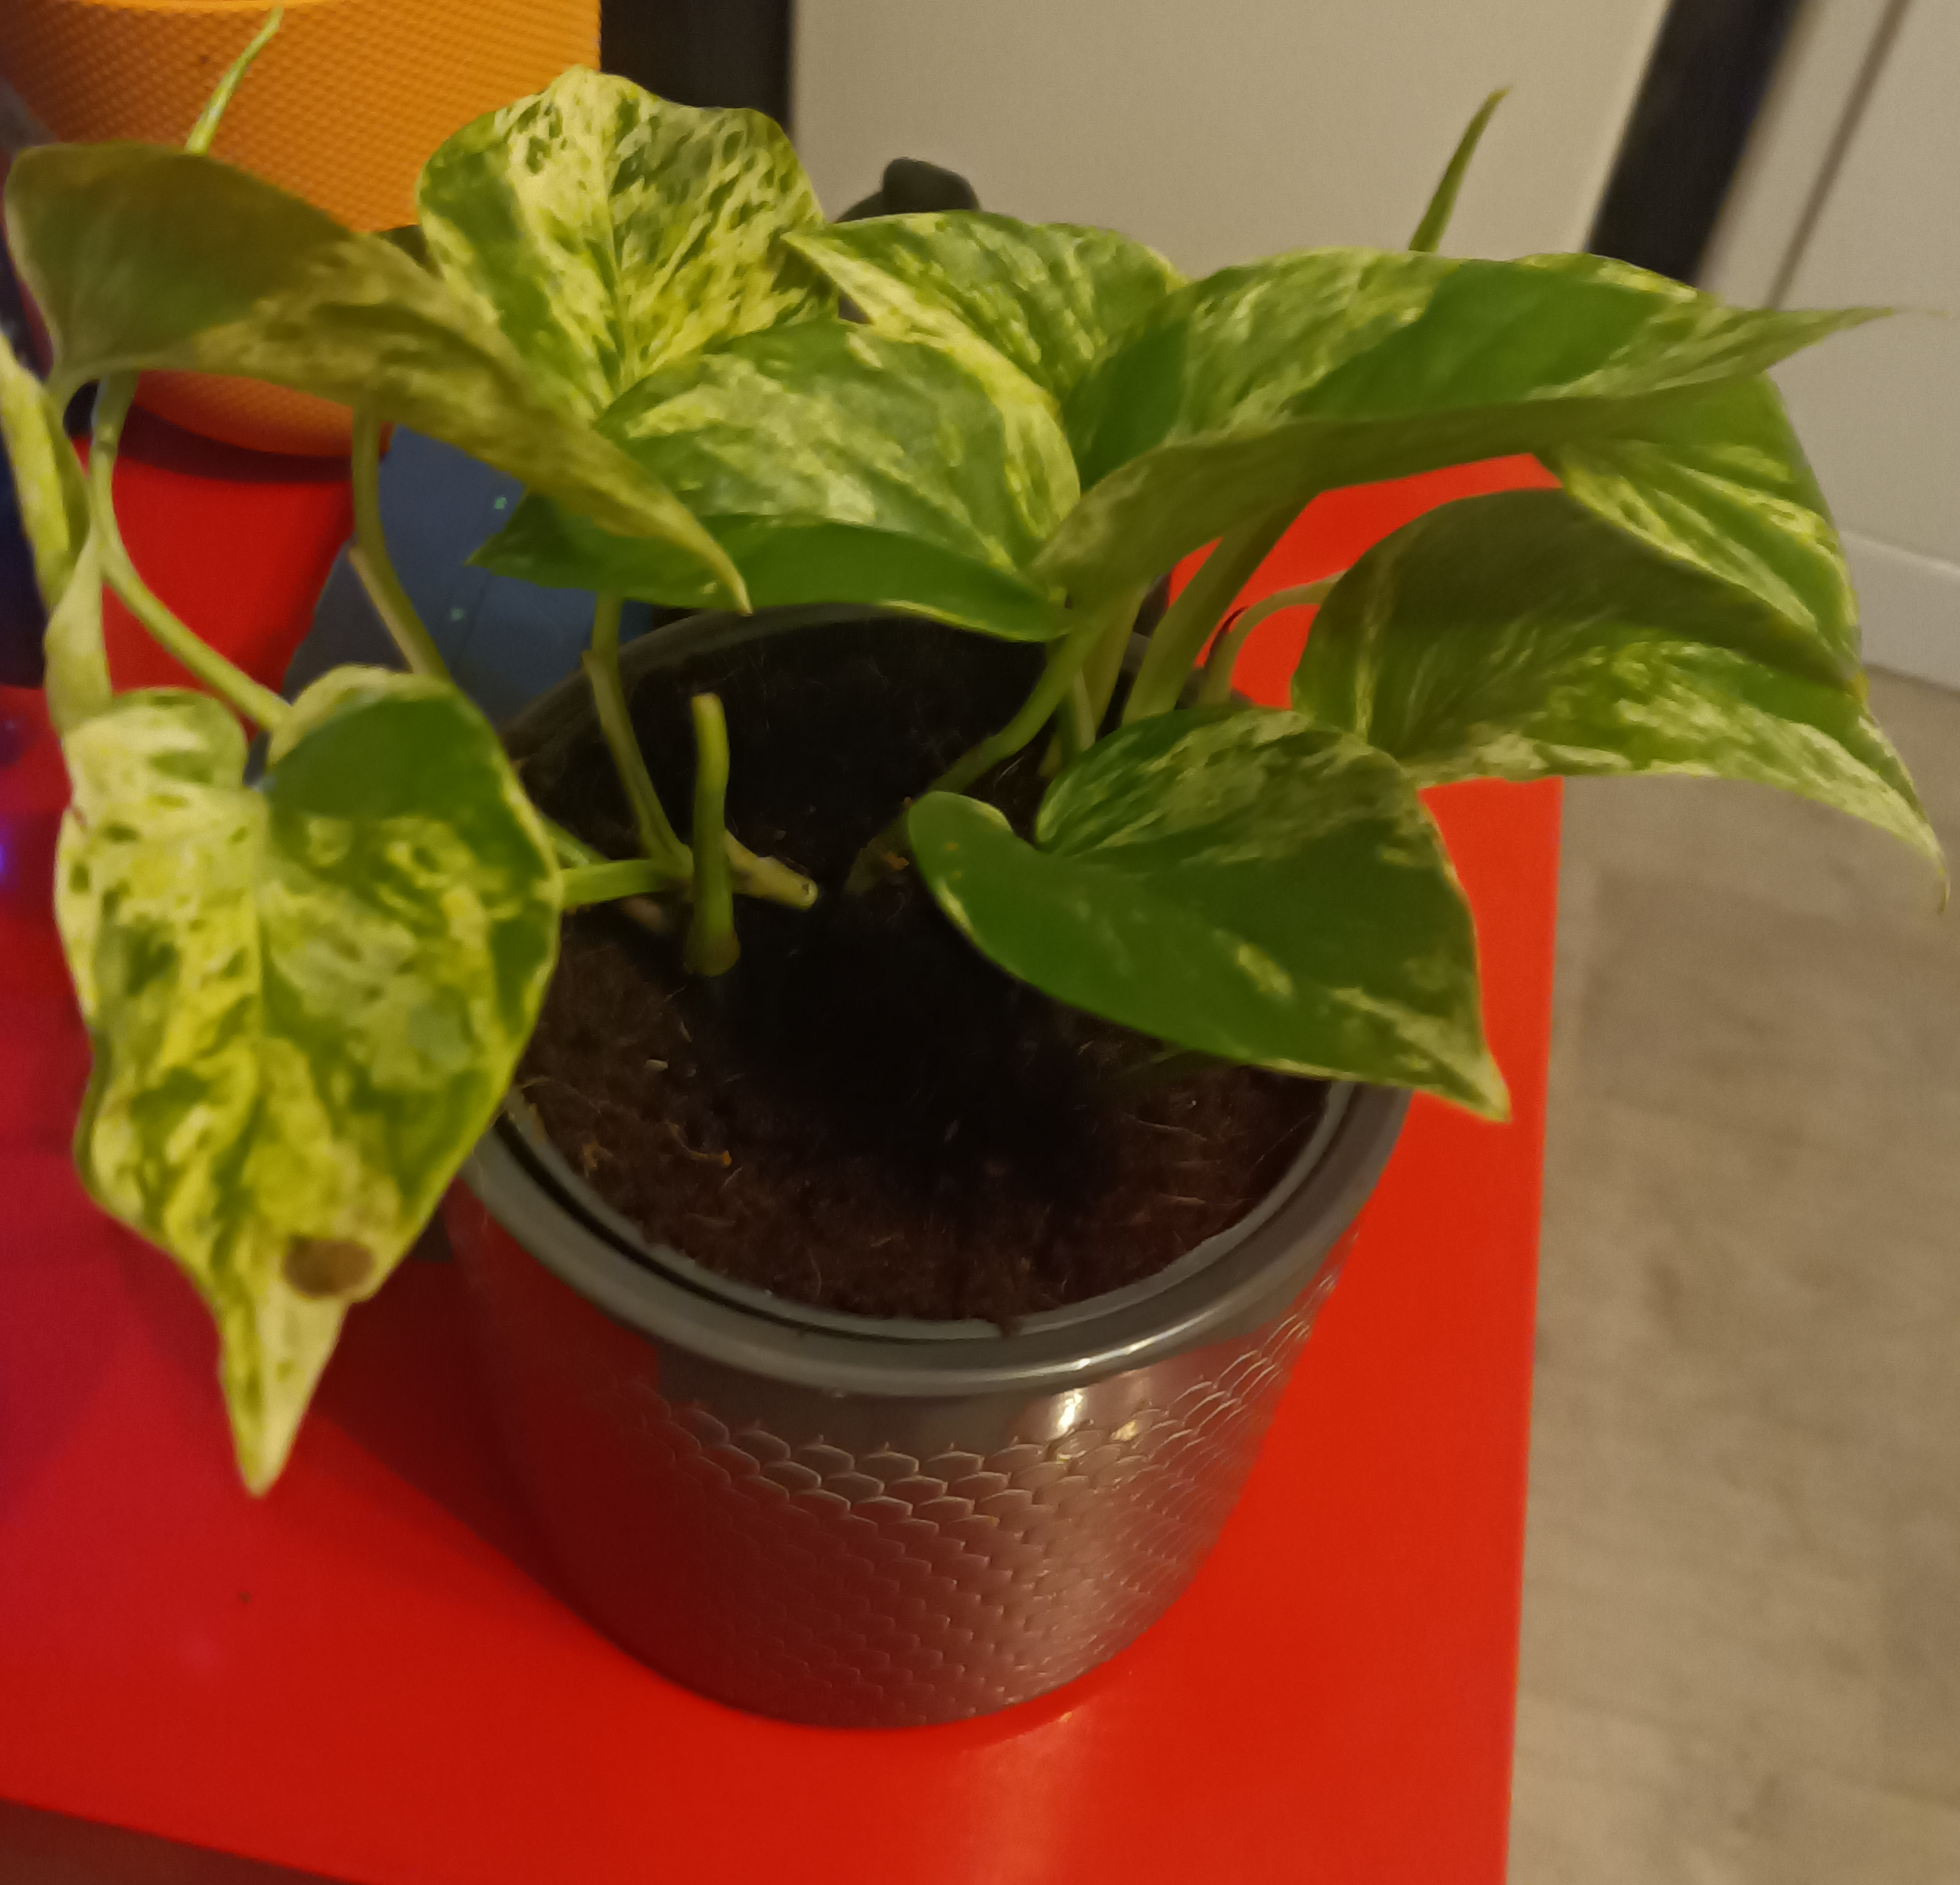
\includegraphics[width=\textwidth]{./images_plantnet/pothos_marble.png}
        \caption*{Observation of a plant which necessitates identification (\textcopyright Tanguy Lefort). The image is sent to Pl@ntNet's computer vision model for identification. A similarity search is performed to present similar pictures for each proposed species.}
    %     \label{fig:image1}
    \end{minipage}
    \hfill
    \begin{minipage}[b]{0.55\textwidth}
        \centering
        \includegraphics[width=\textwidth]{./images_plantnet/pothos_marble_plantnet.png}
        \caption*{Pl@ntNet identification results}
    %     \label{fig:image3}
    \end{minipage}
    \caption{From an image query, Pl@ntNet outputs possible species. For visual aid, close-looking images are also shown for each proposed species. The user can then click on the \emph{compare picture} button to make their choice. Then, the user can vote on the species by clicking on the \emph{It's the right species} button. Here the probability of the \emph{Epipremnum aureum} (Linden \& André) G.S.Bunting to be the right species is $65\%$ -- also known as \emph{Pothos aureus} Linden \& André.}
    \label{fig:pothos_id}
\end{figure}

\subsubsection{Author contribution.}

In Pl@ntNet, an observation is a set of images taken by a user in the field.
The author user can then upload these images to the platform.
The platform will then propose a list of possible species for the observation with the associated predicted probabilities and other images that are close-looking to the picture taken.
The author can then vote on the species they think are present in the observation as illustrated in \Cref{fig:pothos_id}.

The vote is guided by the computer vision model predictions (see \Cref{sub:pipeline_plantnet}) and other pictures selected via a similarity search algorithm.
This similarity search is important as the same species can have different visual presentations at multiple stages of its life cycle.
The similarity search is based on the features from the last layer of Pl@ntNet's network.
These features are hashed using the Random Maximum Margin Hashing algorithm \citep{joly2011random} and then an approximate $k$-nearest neighbors is applied \citep{joly2008posteriori}.

If a user disagrees with the model's predictions, they can enter the name of the species freely in the input box as shown in \Cref{fig:pothos_sharing}.
The user input is guided by the name of possible species in the currently selected flora.

% \begin{wrapfigure}[14]{l}{.55\textwidth}
        \begin{figure}[tbh]
        \centering
        \includegraphics[width=.55\textwidth]{./images_plantnet/free_sharing_pothos.png}
        \caption{The author can select one of the model's predicted species or input freely the name of a species. The user input is guided by the name of possible species in the currently selected flora (here World Flora). Note that by clicking on the gear icon, a user can change the flora.}
        \label{fig:pothos_sharing}
        \end{figure}
% \end{wrapfigure}

The author can also input any text freely -- hence adding possible noisy votes.
At this stage, there is no filter performed on the existence of the given species in the database.
The author can also share the location of the observation, and add additional inputs in a specific reserved field -- the habitat, the aroma or any other feature they would like to share.
Some users unfortunately might mistake the different fields and input information as the species name, a cleaning step is thus a necessary step in the platform.

\subsubsection{Other users contributions.}

Once the observation is shared online, it is time for others to enter the collaborative playground.
Any user can visit the \emph{identify} Pl@ntNet platform and vote on observations.
The view is as presented in \Cref{fig:others_plantnet}.

\begin{figure}[tbh]
        \centering
        \includegraphics[width=.85\textwidth]{./images_plantnet/plantnet_others.png}
        \caption{View of observations as a user (\textcopyright Pavlos). The current prediction is shown, with the initial species proposed. Suggestions from other users are on the right, with a field to propose your thoughts or accept someone else's. Anyone can vote for the organ shown in the image -- in this case, users agree on the flower. The quality is accepted by 2 users and there is no vote to reject the observation based on the fact there is no plant in the actual image.}
        \label{fig:others_plantnet}
\end{figure}

The initial author determination -- if existing -- is shown, with the current prediction.
In the \emph{suggested name} box, all registered species votes are shown with the number of agreements.
In \Cref{fig:others_plantnet}, 5 different users voted: 3 for the species \emph{Vesalea grandifolia} Villarreal Hua Feng Wang \& Landrein, 1 for the \emph{Zabelia triflora} (R.Br. ex Wall.) Makino ex Hisauti \& H.Hara and one user voted for \emph{undertermined} -- meaning they could not identify the species or there is not enough information provided to their knowledge to identify the species.
There is a field for a new vote, where the user is guided to propose an existing species but can enter any text freely.
By clicking on the Pl@ntNet icon next to it, the model's predictions are shown with the associated probabilities and close-looking examples to guide the identification as in \Cref{fig:pothos_id}.

In addition to the species, users (as authors) can vote on the organ shown in the image(s).
The organs can be a leaf, flower, fruit, bark, habit (form in which the plant grows) or other.
Users can approve or disapprove the quality of the image -- if the plant is not correctly visible, the image is blurry, or the organ is not visible.
If there is no plant in the image, they can also flag it with the \emph{no plant} button.

In the upper-right section of the presented observation, the user can see if the observation was associated with any geolocalisation, if the observation is considered as \textbf{valid} by the Pl@ntNet algorithm and if it was reviewed by others.
The \emph{valid} status is given by the Pl@ntNet algorithm presented in \Cref{sub:algo_plantnet} and is a proxy for the quality of the observation.

The iNaturalist platform uses a research grade status to indicate the quality of the observation\footnote{\url{https://www.inaturalist.org/posts/39072-research-grade}}:
\begin{itemize}
        \item there is a picture or recording of sound,
        \item the genus and/or species name of the organism are specified,
        \item the GPS coordinates are associated,
        \item the observation is timed and dated,
        \item the observatory is identified,
        \item there is at least a $2/3$ agreement consensus by users on the identified species.
\end{itemize}
In Pl@ntNet, the data quality is monitored by this \textbf{valid} status that depends on the estimated reliability of a user and the agreement of the community on the observation.
We explain in more detail the algorithm used to estimate the reliability of a user in \Cref{sub:algo_plantnet}.

\subsubsection{What is not an observation.}

Until now, we described what is an observation.
So, let us show examples of what isn't an observation.

\begin{figure}[bth]
        \centering
        \begin{minipage}[t]{0.25\textwidth}
            \centering
            \includegraphics[width=\textwidth,height=4cm]{./images_plantnet/katyykkk_no_plant.png}
            \caption*{A drawing is not a plant (\textcopyright Katyykk)}
        %     \label{fig:image1}
        \end{minipage}
        \hfill
        \begin{minipage}[t]{0.25\textwidth}
            \centering
            \includegraphics[width=\textwidth,height=4cm]{./images_plantnet/eugenio_perez_perez_shroom.png}
            \caption*{A fungus is not in the Plantae kingdom (\textcopyright eugenio perez perez)}
        %     \label{fig:image3}
        \end{minipage}
        \hfill
         \begin{minipage}[t]{0.47\textwidth}
                \centering
                \includegraphics[width=\textwidth,height=4cm]{./images_plantnet/PA0L0_D1_B3LL0_minecraft.png}
                \caption*{A video game tree (Minecraft version of a birch tree) is not a real plant. (\textcopyright PA0L0\_D1\_B3LL0)}
            %     \label{fig:image3}
            \end{minipage}
        \caption{Three examples of images that are not plant observations.}
        \label{fig:not_an_observation}
    \end{figure}

More generally, drawings -- even realistic -- of plants or photos of images of plants are not considered plant observations.
The same goes for fungi, which are not part of the Plantae kingdom and thus are not identified by Pl@ntNet.
Finally, images of video games -- even if they represent plants -- are not considered plant observations.
We show examples of these in \Cref{fig:not_an_observation}.
Photos of people, animals, pornographic images or any other object that is not a plant are also not considered plant observations.
These images are flagged, removed from the platform and are not used to train the models.

Another possible issue is the presence of multiple species in the same observation.
These observations are flagged as \emph{malformed}, we provide an example in \Cref{fig:malformed_observation}.
Users can cast their vote to indicate that the observation is malformed and should not be considered.

\begin{figure}[htbp]
        \centering
        \includegraphics[width=.75\textwidth]{./images_plantnet/maformed_leonardo_liberati.png}
        \caption{Malformed observation: each image is associated with a different species (\textcopyright Leonardi Liberati).}
        \label{fig:malformed_observation}
\end{figure}

\subsection{A step in a bigger pipeline}
\label{sub:pipeline_plantnet}

\begin{figure}[thb]
        \centering
        \includegraphics[width=.65\linewidth]{./images_plantnet/plantnet_schema_global_green.pdf}
        \caption{Pl@ntNet system of human-AI interaction for plant species recognition. Users take their plant observations in the Pl@ntNet application. A prediction is output by the AI model. Users can validate the prediction or propose another species. The whole votes collection is used to evaluate user expertise and actively revise observations identifications.}
        \label{fig:plantnet-system}
    \end{figure}

The gathering and aggregation of votes is only a part of the Pl@ntNet pipeline.
Schematized in \Cref{fig:plantnet-system}, the Pl@ntNet system is a positive loop between curating the data and training a computer vision model.
The label aggregation algorithm is presented in detail in \Cref{sec:aggregation_plantnet}.
Let us briefly address the computer vision model part.

\subsubsection{Model training.}

At the time of writing, the model in use in Pl@ntNet is DINOv2 \citep{oquab2024dinov2} a transformer-based network, trained on Jean-Zay cluster generally every 2 to 3 months\footnote{or sooner if improvements are noticed by J-C Lombardo whom I'm most grateful for the details given about the Pl@ntNet training and testing pipeline.}.
The training steps have evolved in the past years.
In the next paragraphs, we present in a non-exhaustive way the pipeline (presented in \Cref{fig:training_plantnet}) for the current model training.

\begin{figure}[htbp]
    \centering
    \includegraphics[width=\textwidth]{./images_plantnet/training_network.pdf}
    \caption{Pl@ntNet pipeline: the steps to train a neural network from the collaboratively annotated data. The algorithm presented in \Cref{sec:aggregation_plantnet} is used to get labels and a validity indicator. Subsampling and data from partners are then combined to get a labeled dataset to train the current DINOv2 model. Evaluation is performed on the generated test set and additional private test sets.}
    \label{fig:training_plantnet}
\end{figure}

The first step is to gather the data from the Pl@ntNet platform and aggregate the labels as presented later in \Cref{sec:aggregation_plantnet}.
Then, a first cleaning step is performed to remove the noisy labels -- species not in any botanical checklist such as WCVP -- and only keep \textbf{valid observations}. Roughly speaking, valid observations are observations that are considered reliable by the Pl@ntNet algorithm thanks to enough users' expertise and agreement in votes.
In addition to species, the organ is also kept for training.

The data is then cleaned by collected species.
In each species let us consider there are $n_k\in\mathbb{N}$ observations, the valid observations with the most user weight are selected, and then they randomly select $\min(n_k, n)$ observations, with $n\in\mathbb{N}_*$.

On the side, a neural network binary classifier is trained on another dataset to detect if the observation comes from a herbarium or not (binary classification). This classifier is then used to filter out the herbarium observations from the dataset. Herbarium observations are only used for rare species to populate classes with few observations. They are not used if there are \emph{enough} in-the-wild observations as they might.

From the selected observations, the observations constitute a highly imbalanced dataset. This imbalance is necessary as plant species' presence is not balanced in the real world.
Additional data is then collected from partners -- botanic gardens, GBIF, \emph{etc.} -- to get information on organs, species, diseases and other relevant information.
The additional data is not used to balance the dataset, only to provide more information and populate some species -- but the imbalance is kept.
All partner's observations are standardized (resize and compression).

As users can freely upload observations, the observations might not be plant observations (as in \Cref{fig:not_an_observation}).
There are $20$ rejection classes, including but not limited to \emph{homosapiens} (presence of a hand, foot or face), \emph{dogs}, \emph{cats}, \emph{fungi} (presence of a fungus), \emph{no plant} (no plant in the image), \emph{drawing} (presence of a drawing), \emph{screenshot} (the image is not a photo taken by the user), \emph{objects} (presence of an object), \emph{genitalia}, \emph{etc.}
The rejection classes are used to filter out the observations that are not plant observations but also can provide feedback to the user.
For example, if a face is present in the photo taken, the system will warn the user that they might want to retake the photo without the face.
Note that not all rejections provide feedback to the user, some are used to filter out the observations (like the \emph{genitalia} class) and train the Pl@ntNet model to detect images that should not be classified as plants.

The rejection classes are added to the species classes and so is the associated data.
The data is then split into a training, validation and test set.
The test set is about $1\%$ of the filtered data.
The split is stratified by species and organ.
Then the model is trained.

Before the latest model version, the training was done in two steps.
First, the model was trained on species recognition, then frozen, and then finetuned on organ recognition.
Now, the current model is trained directly for multitask classification.
In addition to species and organ recognition, diseases (on plants and crops), the genus, the family and some cultivars (sublevel of taxonomy) of interest for other Pl@ntNet projects are also predicted.
Denoting $\mathcal{L}_{\bigcdot}$ the loss related to the classification task $\bigcdot$, the multitask loss $\mathcal{L}_{\text{multitask}}$ to minimize is of the form:
\[
\mathcal{L}_{\text{multitask}} = \lambda_1 \mathcal{L}_\text{species} + \lambda_2\mathcal{L}_\text{organ} + \lambda_3 \mathcal{L}_\text{genus} + \lambda_4 \mathcal{L}_\text{family} + \lambda_5 \mathcal{L}_\text{disease} + \lambda_5 \mathcal{L}_\text{cultivars} + \dots,
\]
with $(\lambda_p)_p$ the importance weights in the loss, and $\lambda_1 > \lambda_{p'}$ for $p'>1$ as the species determination is the main task for the model.
Let us focus on the species determination as it is the main application of this thesis.
To take into account the imbalance in the dataset, the species determination loss is weighted by the inverse of the class frequency. Note that other losses are also considered in recent work from the Pl@ntNet team \citep{Garcin_Servajean_Joly_Salmon22}.
Transformation on images such as rotation, cropping and flipping are applied.
Label smoothing is used as it is known to improve the uncertainty estimation of the model.

\begin{figure}[htb]
    \centering
    \includegraphics[width=.65\textwidth]{./images_plantnet/cosine_annealing_restart.pdf}
    \caption{Learning rate schedule with a cosine annealing strategy with warm restarts. The learning rate at epoch $t$ depends on the number of epochs in the initial cycle $T_0$ and the cycle length factor $T_{mult}$. The initial learning if $\eta_{\max}=0.1$ and the minimal learning rate is $\eta_{\min}=10^{-3}$.}
    \label{fig:lrscheduler}
\end{figure}

Unlike in \Cref{chap:waum}, the learning rate is scheduled with a cosine annealing strategy with warm restarts \citep{loshchilov2016sgdr} and not a multistep strategy.
Given an initial learning rate $\eta_0=\eta_{\max}>0$, a minimal learning rate $\eta_{\min}>0$, the number of epochs in a cycle $T_0$ and the current number of epochs in  the cycle $T_{curr}$, the learning rate is updated at each iteration $t$ as:
\[
\eta_t = \eta_{\min} + \frac{1}{2}(\eta_{\max} - \eta_{\min})\left(   1+ \cos\left\{ \frac{T_{curr}}{T_0}\pi \right\}\right)    \enspace.
\]

In practice, the cycle size is increased by a factor of $T_{mult}>0$ at each restart -- see \Cref{fig:lrscheduler} for a visualization of the learning rate scheduled with such a scheduler. Thus, denoting $N_{T_{curr}}$ the number of restarts before the current iteration $T_{curr}$, the scheduler becomes:
\[
\eta_t = \eta_{\min} + \frac{1}{2}(\eta_{\max} - \eta_{\min})\left(   1+ \cos\left\{ \frac{T_{curr}}{T_{mult}^{N_{T_{curr}}}T_0}\pi \right\}\right)    \enspace.
\]

This scheduler is known to help improve convergence and performance.
Indeed, the smooth variation helps the optimization process to escape local minima and explore the parameter space more effectively.
Moreover, thanks to the periodic restarts, the model is forced to explore different regions of the optimization landscape. This can prevent the model from getting stuck in suboptimal solutions and encourages better exploration of the parameter space.

\subsubsection{Model evaluation.}

The model is evaluated on multiple test sets.
A first test set is inherited from the train-validation-test stratified split.
It represents $1\%$ of the data and is used to check the performance on Pl@ntNet and the partner's data.
Other test sets are used to evaluate the model on specific tasks and species recognitions.
Those safe sets contain unreleased and curated data that are only to be used for the evaluation of this model.

\subsubsection{On the model characteristics.}

The current Pl@ntNet model -- DINOv2 \citep{oquab2024dinov2} -- is a transformer-based network \citep{dosovitskiy2020image}.
The former models used were a BEiT \citep{bao2021beit} -- also transformer-based -- and an InceptionV3 \citep{szegedy2015rethinking} -- a convolutional neural network.
Hereafter, we briefly describe the DINOv2 model characteristics.

In essence, the DINOv2 model is part of the DINO family: a family of models that combines self-supervised learning and knowledge distillation.
More details about DINOv2 are available in the original paper \citep{oquab2024dinov2} and the work before \citep{caron2021emerging}.

On one hand, knowledge distillation is performed by training a student model to mimic a teacher model. Given an input image, both networks predict a feature embedding vector and the KL divergence loss between the two predictions is minimized.
On the other hand, the self-supervised aspect allows the training of a network without labels first and then finetuning it on a supervised dataset.
To achieve this, contrastive learning is used: the goal is for the model to minimize the distance between similar pairs of data and maximize the distance for dissimilar ones.

So how does DINOv2 combine both concepts? First, note that the contrastive learning step is hidden in the embedding representation of the images \citep{caron2020unsupervised}. Then, we can simplify DINOv2 into three main objectives:
\begin{itemize}
    \item Image-level objective: cropped images are fed to a ViT-H/16 transformer -- a vision transformer that divides images into $16$ patches ($4\times 4$ grid) that is pretrained here on the ImageNet-22K dataset -- to produce embeddings. The student network is trained on the embeddings to mimic the teacher network.
    \item Patch-level objective: The DINO teacher network only sees the image-level embeddings. The student network is trained to predict the teacher's embeddings from both the image and the patches' embeddings. This forces the student to learn helpful parts of the image to predict the teacher's embeddings.
    \item Additional objectives: several (non-exhaustively) other regularization terms are added to the objective such as KoLeo regularization of $\ell_2$ normed embeddings from the same batch to spread them uniformly in the feature space, Sinkhorn-Knopp batch normalization (used but not necessary considering their ablation study) \emph{etc}.
\end{itemize}
Note that, we consider embeddings, but a final softmax operator is used to consider distributions and compute cross-entropy loss between teacher and student predictions. However, as both networks do not have access to class labels yet, cross-entropy minimization is done to align the teacher and student embeddings.
Note that additional tricks are performed to prevent the teacher and student networks from collapsing. There are four main tricks used:
\begin{itemize}
    \item Untying weights: as the model head is much smaller than the patch-level architecture, the head can overfit the image-level data while the patches are underfitted. Untying the weights of the head and the patch-level architecture helps to prevent this.
    \item resolution adaptation during training to prevent the loss of small objects, this is especially important in Pl@ntNet as small details on plants can help differentiate species. Note that Pl@ntNet images use a $518\times 518$ resolution.
    \item EMA (exponential moving average): to stabilize the teacher network and prevent collapsing predictions from the student, the teacher network is an exponentially weighted average of the student. Roughly, the update at epoch $t$ of DINOv2's teacher weights is $\theta_t \gets \lambda \theta_t + (1-\lambda)\theta_{s}$ with $\lambda>0$ exponential weight (that follows a cosine schedule from $0.996$ and $1$ during training), $\theta_t$ the teacher weights and $\theta_s$ the student's.
    \item centering and sharpening: both tricks -- while intuitively opposing -- can help avoid collapsing to uniform or Dirac distributions in the feature space. Centering the teacher embeddings before the softmax operator helps to prevent one feature from dominating the others. Sharpening is done by scaling the teacher's embeddings in the softmax. Intuitively, the teacher has access to the full image and thus should be more confident than the student who mostly sees patches. Thus the teacher distribution should peak for the current (unknown) target class. By combining both, the teacher's distribution is non-trivial. This allows Pl@ntNet's network to keep some uncertainty in the predictions.
\end{itemize}

Finally, once this self-supervised learning is done, the model is finetuned on the Pl@ntNet dataset with aggregated labels and can identify plant species and more.
Note that some patch-level operations were removed in Pl@ntNet in order not to classify an image based on a single patch -- \emph{e.g.} an image of a flower next to a genitalia should not be classified as a flower, but a rejection.
The next step in this thesis is thus to detail the label aggregation strategy, compare it to existing (and scaling) ones, and propose ways to improve it.

\section{Pl@ntNet's label aggregation strategy}
\label{sec:aggregation_plantnet}

As we discussed in \Cref{sec:introducing_plantnet}, plant species identification is a task that requires skills to recognize morphological traits (shapes, measurements, environments and specific characteristics).
A large number of users with diverse skills have participated in gathering plant observations and helped improve the training dataset of our computer vision model.
Their participation is based on votes that they can cast on others' observations, or by the initial species determination of their observation.
The quality of each vote is then processed by the algorithm presented in \Cref{sub:algo_plantnet}.

At the time of writing, this participatory approach has resulted in the collection of over 20 million observations, belonging to almost $\numprint{46000}$ species, by more than 6 million users worldwide. In total, more than $25$ million of images are shared in these observations.

Other citizen science projects such as iNaturalist \citep{van2018inaturalist} or eBird \citep{sullivan2009ebird} use a similar approach to collect data, but differ in their label aggregation strategy.
The iNaturalist project, with more than $2.5$ million users, records the votes at different taxonomic levels.
The resulting label is the aggregation of at least two votes on a species-level identification (or coarser or finer taxonomic level).
A taxon requires at least two-thirds agreements among identifiers and all users have the same weight in the decision-making.
Over time, a taxon can be further refined by the community, debated or revoked.
eBird handles taxon quality control by using a checklist in each region for observers.
Quality control on the checklist is performed and, combined with user knowledge -- number of species and checklist submitted, number of flagged observations, discussions among local experts -- the species observation is accepted.
The eBird project also showed that monitoring species accumulation from observers can help to sort their skills \citep{kelling2015}. While they consider the species accumulation by hours spent on each collected observation, we present a strategy that takes into account the entire history of observations of the observer.


\subsection{Presentation of the algorithm}
\label{sub:algo_plantnet}

\begin{algorithm}[h]
        \caption{Pl@ntNet iterative weighted majority vote}
        \label{alg:plantnet_algorithm}
        \textbf{Input}: Votes as $(j, y_i^{(j)})_{i\in [n_{\texttt{task}}],j\in [n_\text{user}]}$ for each observation $x_i\in\mathcal{X}$ and user $j$ answering the voted species $y_i^{(j)}$, accuracy threshold $\theta_{\text{acc}}$, confidence threshold $\theta_{\text{conf}}$, weight function $f$, initial weight $\gamma>0$ \\
        \textbf{Ouptput}: Estimated labels $\hat y_i$ and validity indicator $s_i$ for each observation $i$
        \begin{algorithmic}[1]
            \STATE $\text{Initialize } \hat y_i = \mathrm{MV}\left(\{y_i^{(j)}\}_j\right) \text{ for each observation } i \in [n_{\texttt{task}}]$
            \STATE $\text{Initialize user weights as } w_j = \gamma \text{ for each user } j \in [n_\text{user}]$
            \WHILE{$\text{not converged}$}
                \FOR{each observation $i\in [n_{\texttt{task}}]$}
                    \STATE Compute label confidence: $\mathrm{conf}_i(\hat y_i) = \sum_{j\in \mathcal{A}(x_i)} w_j \mathds{1}(y_i^{(j)}=\hat y_i)$
                    \STATE Compute label accuracy: $\mathrm{acc}_i(\hat y_i) = \mathrm{conf}_i(\hat y_i) / \sum_{k\in [K]} \mathrm{conf}_i(k)$
                    \STATE Compute validity indicator: $s_i = \mathds{1}( \mathrm{acc}_i(\hat y_i) \geq \theta_{\text{acc}} \text{ and } \mathrm{conf}_i(\hat y_i) \geq \theta_{\text{conf}})$
                \ENDFOR
                \FOR{each user $j \in [n_\text{user}]$}
                    \STATE Compute the number of valid identified species for authoring observations: \[n_j^\text{author} = |\{y_i^{(j)}\in [K] \,|\, y_i^{(j)}=\hat y_i, s_i=1, \mathrm{Author}(i)=j\}|\]
                    \STATE Compute the number of identified species by voting on other's observations: \[n_j^\text{vote}=|\{y_i^{(j)}\in [K]\,|\, y_i^{(j)}=\hat y_i, \mathrm{Author}(i)\neq j\}|\]
                    \STATE Compute the rounding number of identified species per user: \[n_j = \mathrm{Round}\left(n_j^\text{author} + \frac{1}{10}n_j^\text{vote}\right)\]
                    \STATE Transform number of estimated species per user into trust score: $w_j = f(n_j)$
                    \ENDFOR
                \STATE Update estimated labels with a weighted majority vote $$ \forall i \in [n_{\texttt{task}}],\ \hat y_i = \argmax_{k\in[K]} \sum_{u\in \mathcal{A}(x_i)} w_j\mathds{1}(y_i^{(j)}=k)$$
            \ENDWHILE
        \end{algorithmic}
    \end{algorithm}

Pl@ntNet label aggregation strategy relies on estimating the number of correctly identified species for each user.
Similar to other strategies, we rely on an EM-based iterative procedure \citep{Dempster_Laird_Rubin77} to estimate consecutively the users' skills and each observation's species. The detailed iterative algorithm is provided in \Cref{alg:plantnet_algorithm}.

The label aggregation strategy generates a trust indicator ($s_i$) on the observation that can reveal whether an observation is valid or not.
Notice that in \Cref{alg:plantnet_algorithm} we value $10$ times more authored observations than voting on other's observations -- if a user proposes a new observation with a label (species name) it is more useful than proposing a label by clicking.
Indeed, being on the field leads to more information on the environment and a better determination of the species.
Finally, note that an identified species is exclusively identified as an author -- part of $n_j^\text{author}$ in \Cref{alg:plantnet_algorithm} -- or as click -- part of $n_j^\text{vote}$ -- to avoid redundant skills.
%species are unequivocally identified as authors ($n_u^\text{author}$ in \Cref{alg:plantnet_algorithm}) or as votes on other's observations ($n_u^\text{vote}$).
The final number of species identified by users is the aggregation of these two terms: $n_j = \mathrm{Round}\left(n_j^\text{author} + \frac{1}{10}n_j^\text{vote}\right)$.

\begin{figure}[htb]
    \centering
    \includegraphics[width=.75\textwidth]{./images_plantnet/weight_function.pdf}
    \caption{Weight function in \Cref{eq:weight_func} used to map the number of identified species to a trust score in the Pl@ntNet label aggregation strategy. A new user starts with a weight of $f(0)=f(1)=\gamma\simeq 0.74$. The user confidence threshold $\theta_{\text{conf}}=2$ requires a user to have identified at least $n_j=8$ species to become \textbf{self-validating}. The parameters $\alpha=0.5$, $\beta=0.2$ and $\gamma\simeq 0.74$ are used in practice.}
    \label{fig:weight_function}
\end{figure}

The weight function $f$ shown in \Cref{fig:weight_function} is a non-decreasing function that maps the number of identified species $n_j$ to a trust score in the form of:
\begin{equation}\label{eq:weight_func}
    w_j = f(n_j) = n_j^\alpha - n_j^\beta + \gamma \enspace,
    \end{equation}
where $\alpha,\beta\in\mathbb{R_+^\star}$ are hyperparameters that were calibrated internally to fit prior knowledge and $\gamma>0$ is the constant representing the initial weight of each user. In practice, we use $\alpha=0.5$, $\beta=0.2$ and $\gamma=\log(2.1)\simeq 0.74$ in the weight function.
This function is sub-linear ($\mathcal{O}(\sqrt{n_j}))$ but with two regimes.
The goal of \Cref{eq:weight_func} is to separate new users from experts and then help sort multiple experts.
This is modeled by the two regimes of the weight function.
In the first regime which corresponds to new users with low $n_j$, the term in the power of $\beta$ decreases the weight. We chose an initial weight $w_j=\gamma$ such that a user has a weight equal to $1$ (rounding to two decimals) with two different identifications. This separates the users who only come once to test the application from others.
In the second regime with a higher number of identified species, the term to the power of $\beta$ becomes negligible and we tend to the square root function.
The sub-linear scale allows for reducing discrepancies between people who have identified a comparable number of species (and thus have presumably comparable expertise).
As for the two thresholds that control the level of uncertainty accepted for a given label, they are set to $\theta_{\text{conf}}=2$ to control the total weight on an observation and $\theta_{\text{acc}}=0.7$ to control the agreement between users given their expertise.

Users are said \textbf{self-validating} when they are trusted enough so that their proposed label single-handedly makes an observation valid $(s_i=1)$.
From \Cref{alg:plantnet_algorithm}, we see that this is verified when their weight $w_j$ is greater than the level $\theta_{\text{conf}}$.
Indeed, with a single label we obtain $\mathrm{conf}_i(\hat y_i) = w_j > \theta_{\text{conf}}$ and $\mathrm{acc}_i(\hat y_i) = 1 > \theta_{\text{acc}}$.
In practice, this means that an experienced user who has collected enough weight can validate any observation without any other user's vote.
Note that this identification can later be invalidated by other users with enough weight thanks to the accuracy threshold $\theta_{\text{conf}}$.

\subsection{Introducing a subset of Pl@ntNet to evaluate the current strategy}

To compare the different label aggregation strategies on large-scale datasets, we introduce a subset of the Pl@ntNet database focused on Southwestern European flora observations -- Baleares, Corsica, France, Portugal, Sardegna and Spain -- from $2017$ to October $2023$.
In total, $\numprint{9005108}$ votes are cast by $n_\text{user}=\numprint{823251}$ users on $\numprint{6699593}$ observations after two cleaning steps on the voted species.
The first one is a filtering step. We only keep the votes with plant species belonging to the World Checklist of Vascular Plants (WCVP) \citep{govaerts2023world}.
For the second step, according to Kew's Royal Botanical Garden, we matched synonyms to their backbone species if the species is part of the \emph{k-southwestern-europe} checklist from Plants of the World Online \citep{powo2024} (POWO) system.
% We restrict synonyms to be part of the \emph{k-southwestern-europe} from Plants of the World Online \citep{powo2024} (POWO) system.
Note that there are plant species listed in the accepted species from WCVP that are not in the \emph{k-southwestern-europe} POWO checklist.
As there is a possible taxon ambiguity in this case -- multiple species possible for a given synonym depending on the referential  -- we leave the proposed label untouched.
The dataset is available at \url{https://zenodo.org/records/10782465}.

In the following, denote $K$ the number of species within the dataset.
We will consider multiple subsets of one large released dataset.
We index the observations by $i\in [n_{\bigcdot}]=\{1,\dots,n_{\bigcdot}\}$ where $\mathcal{D}_{\bigcdot}$ is the considered dataset composed of $n_{\bigcdot}$ observations and their associated votes.
For a given subset we do not address the number of observations (previously called tasks) as  $n_\texttt{task}$ but as $n_{\bigcdot}$.
For example, the full south-western European flora dataset from Pl@ntNet of $n_{\mathrm{SWE}}=\numprint{6699593}$ observations is denoted $\mathcal{D}_{\mathrm{SWE}}$.
Other subsets are presented in \Cref{fig:sankey}.
Each user $j$ has a unique identifier used as an index, and we denote $\mathcal{A}(x_i)$ the set of users that have voted on observation $x_i$.
The vote of user $j$ on observation $i$ is denoted $y_i^{(j)}\in [K]$ is a free text field.
Estimated labels are denoted $\hat y_i \in [K]$ -- we only consider hard labels.
Each observation $i$ is created by an author $j$ stored in $\mathrm{Author}(i)$.

\begin{figure}[tbh]
    \begin{center}
        \includegraphics[width=\textwidth]{./images_plantnet/sankey_v2.pdf}
    \end{center}
    \caption{Log-scales distribution of the observations in the South-West European Flora subset from the Pl@ntNet database. Note that the (sub-)datasets introduced are nested: $\mathcal{D}_{\mathrm{SWE}} \supset \mathcal{D}_\text{expert} \supset \mathcal{D}_{\text{multiple votes}} \supset \mathcal{D}_{\text{disagreement}}$. $\mathcal{D}_{\text{expert}}$ and the following subsets contain observations that received at least one vote from one of the experts.}
    \label{fig:sankey}
\end{figure}

\subsubsection*{Creation of an evaluation set in a crowdsourcing setting.}

To evaluate the performance of a label aggregation strategy, it is necessary to know the ground truth on a subset of the data.
However, in the context of crowdsourced data, there is no known truth for the observations.
The sheer volume of data makes it impossible to ask botanical experts to create such ground truth for the whole database.
Moreover, identifying species from images is much less accurate than identifying them in the field, due to the partial information contained in the image \citep{experts2018plant}.

Instead of asking experts to label a subset of the data, we rather identify botanical experts in the Pl@ntNet user database and consider their determinations as ground truth.
We asked botanical-known experts to reference other experts who could have a Pl@ntNet account to create a list of expert users.
To these we have added TelaBotanica \citep{heaton2010tela} users with registered confirmed botanical experience from their account and that are also Pl@ntNet users that participated in the South-Western Europe flora subset.
In total, $98$ Pl@ntNet users were identified as botanical experts.
Observations with at least one vote from one of these experts constitute our test set denoted $\mathcal{D}_\text{expert}$.
The answers of these experts are considered ground truth labels and used to evaluate strategies' performance.
Despite our selection process of supposedly `indisputable' experts, a few observations in the test set still end up with contradictory labels ($4$ observations in total). As they represent a very small percentage, we simply removed them from $\mathcal{D}_\text{expert}$.

\begin{figure}[htb]
    \centering
    \begin{subfigure}[t]{.52\textwidth}
        \centering
        \includegraphics[width=\linewidth]{./images_plantnet/obs_species_per_user.pdf}
        \caption{Relationship between the number of observations per user and the variety of species proposed per user. Each point represents a concentration of users in the SWE flora subset. $\numprint{310,564}$ users proposed a single vote.}
        \label{fig:users_obs_species}
    \end{subfigure}%
    \hfill
    \begin{subfigure}[t]{.40\textwidth}
        \centering
        \includegraphics[width=\linewidth]{./images_plantnet/lorenz_curves.pdf}
        \caption{Lorenz curves representing the imbalance distribution of the number of votes in the South-West European Flora subset from the Pl@ntNet database. This imbalance is mitigated but kept in the created test set.}
        \label{fig:lorenz}
    \end{subfigure}
    \caption{Pl@ntNet activity summary in the SWE flora subset. (A): The majority of users have proposed a small number of observations and species. However, some users have proposed a large number of observations and species. (B): In a perfectly balanced dataset, the Lorenz curve would be the diagonal -- $50\%$ of the votes would be for $50\%$ of the observations. In practice, there is a high imbalance of the distribution of votes between observations -- $80\%$ of the observations are represented by $10\%$ of votes. In total, $5.90\%$ of the users are \textbf{self-validating}($\numprint{50446} users in SWE flora subset$).}
    \label{fig:summary_subset}
\end{figure}

Our evaluation set $\mathcal{D}_{\text{expert}}$ is finally composed of $\numprint{26811}$ observations which received at least one vote from one of the experts.
Despite the large number of users, not all observations obtain multiple annotations.
Indeed, $\numprint{310564}$ users were single-time voters (meaning they interacted with the system only once).
The lack of votes is a large component of difficulty in the Pl@ntNet database, as there is a high imbalance of the distribution of votes between observations as represented in \Cref{fig:lorenz}.
There is a high concentration of votes for a small percentage of the observations as shown in \Cref{fig:users_obs_species}.
Of these evaluation data, $\numprint{17125}$ received more than two identifications and are stored in $\mathcal{D}_{\text{multiple votes}}$.
Then, $\numprint{1263}$ have more than two votes with at least one disagreement between users and are stored in $\mathcal{D}_{\text{disagreement}}$.
\Cref{fig:sankey} shows the distribution of observations from $\mathcal{D}_{\mathrm{SWE}}$ to the finer and more ambiguous $\mathcal{D}_{\text{disagreement}}$.

\subsubsection*{Evaluated aggregation strategies.}

Plant species label aggregation is a challenging task due to the large number of species $K=\numprint{11425}$.
Hence, many classical strategies in the label aggregation literature such as Dawid and Skene's \citep{dawid_maximum_1979} and other variations \citep{passonneau-carpenter-2014-benefits, sinha2018fast} are not applicable as they require estimating a $K\times K$ confusion matrix for each user.
For the considered dataset $\mathcal{D}_\text{SWE}$, this would result in $\numprint{11425}^2\times \numprint{823251}\approx 10^{14}$ parameters to estimate.
Similar issues occur for other label aggregation strategies \citep{whitehill_whose_2009,hovy2013learning,ma2020adversarial}.
We do not consider deep-learning-based crowdsourcing strategies as \citet{rodrigues2018deep,chu2021learning} or \citet{lefort2022improve} as they require training a neural network from crowdsourced labels, but do not output aggregated labels on the training set.
In the Pl@ntNet application, we need to propose one or multiple species for each observation to users.
To overcome these issues, we consider the following label aggregation strategies that can scale with $K$ and the number of users:
\begin{itemize}
    \item \textbf{Majority Vote (MV)}: it selects the most answered label and is the most common aggregation strategy. More formally, given an observation $i$:
    \[\mathrm{MV}(i, \{y_i^{(j)}\}_j) = \argmax_{k\in [K]} \sum_{j\in\mathcal{A}(x_i)} \mathds{1}(y_i^{(j)} = k) \enspace.\]
    \item \textbf{Worker Agreement With Aggregate (WAWA)}: this strategy, also known as the inter-rater agreement, weights each user by how much they agree with the MV labels on average. More formally, given an observation $i$:
    \begin{align*}
        \mathrm{WAWA}(i, \mathcal{D}_{\mathrm{SWE}}) &= \argmax_{k\in [K]} \sum_{j\in\mathcal{A}(x_i)} w_j\mathds{1}(y_i^{(j)} = k) \\
        \text{with } w_j &= \frac{1}{|\{y_{i'}^{(j)}\}_{i'}|} \sum_{i'=1}^{n_{\mathrm{SWE}}} \mathds{1}\left(y_{i'}^{(j)} = \mathrm{MV}(i',\{y_{i'}^{(j)}\}_j)\right)\enspace.
        \end{align*}
    As there is no observation filter for the $\mathrm{MV}$ and $\mathrm{WAWA}$, we consider that for all observation $i$, $s_i=1$ for these two strategies.

    \item \textbf{TwoThird}: The TwoThird aggregation generates a label for observations with at least two votes. The estimated label represents the one with at least two-thirds of the majority in agreement. Every user has the same weight in the aggregation. It is part of the iNaturalist's label aggregation system \citep{van2018inaturalist}. More formally:
    \begin{align*}
        \mathrm{TwoThird}(i, \{y_i^{(j)}\}_j) &= \begin{cases}
            \mathrm{MV}(i, \{y_i^{(j)}\}_j) & \text{if } s_i=1  \\
            \text{undefined} & \text{otherwise} \end{cases}
            \\ \text{ with } s_i &= \mathds{1}\left(\displaystyle\max_{k\in[K]}\frac{1}{|\mathcal{A}(x_i)|}\sum_{j\in\mathcal{A}(x_i)} \mathds{1}(y_i^{(j)}=k) \geq \frac{2}{3}\right) \enspace.
    \end{align*}
\end{itemize}

\subsubsection{Evaluation metrics.}

To evaluate the label aggregation strategies, we use the following label recovery accuracy computed on the evaluation datasets:
\begin{equation*}
    \mathrm{Acc}(\hat y, y; \mathcal{D}_{\bigcdot}) = \frac{1}{n_{\bigcdot}} \sum_{i=1}^{n_{\bigcdot}} \mathds{1}(\hat{y}_i = y_i)\mathds{1}(s_i=1) \enspace,
\end{equation*}
with $\hat y=(\hat{y}_i)_i$ the estimated labels on $\mathcal{D}_{\bigcdot} \in \{\mathcal{D}_\text{expert}, \mathcal{D}_{\text{multiple votes}}, \mathcal{D}_{\text{disagreement}}\}$, $y=(y_i)_i$ the associated experts labels, considered as ground truth.
When the aggregation strategy indicates the observation as invalid ($s_i=0$ for Pl@ntNet and TwoThird), this metric considers the sample as wrongly classified.
Precision and recall scores are also computed to respectively measure the correctness of the observations indicated as valid and the ability to recover the ground truth observations in the valid set.
We take into account the species imbalance by using a macro-average for these metrics. This treats rare species as equally important to common ones. Denoting respectively $\mathrm{TP}_k$, $\mathrm{FP}_k$ and $\mathrm{FN}_k$ the true positives, false positives and false negatives related to the species $k$, the macro averaged precision and recall write
\[
\mathrm{Precision}_{\mathrm{macro}}=\frac{1}{K}\sum_{k=1}^K \frac{\mathrm{TP}_k}{\mathrm{TP}_k + \mathrm{FP}_k} \quad \text{and} \quad \mathrm{Recall}_{\mathrm{macro}}=\frac{1}{K}\sum_{k=1}^K \frac{\mathrm{TP}_k}{\mathrm{TP}_k + \mathrm{FN}_k} \enspace.
\]

As both the Pl@ntNet and the TwoThird strategies can invalidate some of the observations, we also compute the proportion of observations removed from the whole dataset (whereas previous metrics are computed on the evaluation dataset). This complementary metric allows measuring the proportion of samples "lost" for the training of the AI model after the aggregation step.
In practice, filtering data might remove some noisy samples from the dataset. Yet, in general, the more samples are filtered, the fewer ones to train the neural network training.
Finally, we also consider the proportion of species retrieved by the aggregation strategies on $\mathcal{D}_\text{expert}, \mathcal{D}_{\text{multiple votes}}$ and $\mathcal{D}_{\text{disagreement}}$. This is a critical consideration because if a species identified by experts is absent from the aggregated data, the neural network trained on this data will be unable to make predictions for that very species.

We evaluate the label recovery $\mathrm{Acc}$ of each strategy on $\mathcal{D}_\text{expert}, \mathcal{D}_{\text{multiple votes}}$ and $\mathcal{D}_{\text{disagreement}}$ (see also \Cref{fig:sankey}): the test set where experts have provided at least one vote ($\mathcal{D}_\text{expert}$), its subset of observations with at least $2$ votes and one from an expert ($\mathcal{D}_\text{multiple votes}$) and its subset of observations with at least $2$ votes, one from an expert, and one disagreement ($\mathcal{D}_\text{disagreement}$).
The latter is the most challenging as it contains the observations with the most ambiguity.
We selected these subsets to investigate the label aggregation strategies' performance depending on the ambiguity level.

\subsection{Results on label aggregations}
\label{sub:plantnet_res_aggregations}


\begin{figure}[tbh]
    \centering
    \begin{subfigure}[t]{.48\textwidth}
        \centering
        \includegraphics[width=\linewidth, height=5cm]{./images_plantnet/accuracy_by_vol_class_kept_two_votes__micro.pdf}
        \caption{Accuracy on $\mathcal{D}_{\text{multiple votes}}$ w.r.t. to the proportion of classes recovered}
        \label{fig:accuracy_vol_class_multiple}
    \end{subfigure}%
    \hfill
    \begin{subfigure}[t]{.48\textwidth}
        \centering
        \includegraphics[width=\linewidth, height=5cm]{./images_plantnet/accuracy_by_vol_class_kept_one_disagreeement__micro.pdf}
        \caption{Accuracy on $\mathcal{D}_{\text{disagreement}}$ w.r.t. the proportion of classes recovered}
        \label{fig:accuracy_vol_class_disagreeing}
    \end{subfigure}
    \caption{Accuracy of the aggregation strategies w.r.t. the proportion of classes (species) retrieved on subsets with at least two votes -- either agreeing (A) or with at least one disagreeing vote (B). The Pl@ntNet aggregation is more accurate, especially in a highly ambiguous setting (B). The TwoThird data filter highly impacts how many classes are kept in the dataset and the overall accuracy in both settings. WAWA and MV perform similarly with a benefit for WAWA when skill evaluation is needed.}
    \label{fig:accuracy_volume}
\end{figure}

\subsubsection{Accuracy of the aggregation strategies.}

\begin{figure}[htb]
    \centering
    \begin{subfigure}[t]{.48\textwidth}
        \centering
    \includegraphics[width=\textwidth]{./images_plantnet/precision_and_recall_one_disagreeement__macro.pdf}
    \caption{Precision and recall of label aggregation strategies on $\mathcal{D}_\text{disagreement}$. }
        \label{fig:precision-recall}
    \end{subfigure}%
    \hfill
    \begin{subfigure}[t]{.48\textwidth}
        \centering
    \includegraphics[width=\textwidth]{./images_plantnet/volume_train_data.pdf}
    \caption{Number of observations in $\mathcal{D}_{\mathrm{SWE}}$ indicated as valid for training ($s_i=1$). }
    \label{fig:vol_train_data}    \end{subfigure}
    \caption{(A): TwoThird strategy has better precision than MV and WAWA strategies, with lower recall because of the heavy filter on the validity of observations. Pl@ntNet aggregation strategy obtains the best precision and recall and outperforms other strategies. (B): TwoThird performance drop can be explained in part by the high proportion of data considered invalid. Note that MV and WAWA strategies do not invalidate any observation, hence keeping potentially mislabeled or low-quality observations. Pl@ntNet achieves a balance between filtering out observations and achieving high performance.}
    \label{fig:precision-volume}
\end{figure}

We begin by evaluating the accuracy of the label aggregation strategies on the set of observations labeled by experts, $\mathcal{D}_\text{expert}$. \Cref{fig:accuracy_volume} shows how many predicted labels match the experts answers on $\mathcal{D}_{\text{multiple votes}}$ and $\mathcal{D}_{\text{disagreement}}$.
More importantly, we compare this quantity with the proportion of species retrieved by the aggregation strategy.
We observe that the data filtering from the TwoThird strategy -- requiring at least two third of agreements -- highly degrades performance with respect to other strategies.
On $\mathcal{D}_{\text{expert}}$, MV reaches $97\%$ of accuracy, WAWA $98\%$, TwoThird $60\%$ and Pl@ntNet $99\%$.
To differentiate between the best-performing strategies, we need to look at more ambiguous observations like those in $\mathcal{D}_{\text{multiple votes}}$ and $\mathcal{D}_{\text{disagreement}}$.
In highly ambiguous frameworks, the WAWA strategy outperforms the MV one.
However, overall the Pl@ntNet aggregation is more often in adequation with the experts and retrieves almost $90\%$ of plant species identified by experts in highly ambiguous datasets against $73\%$ for WAWA, $71\%$ for MV and only $41\%$ for TwoThird.

\subsubsection{Precision and recall.}

To better evaluate each aggregation strategy, we compute the macro precision and recall metrics for each species. Results are shown in \Cref{fig:precision-recall}. The observations filter ($s_i=0$) for the TwoThird strategy highly impacts its ability to identify most of the positive observations for a given species. While this agreement threshold filter is created to keep as few noisy samples as possible in research-graded (data quality indicator for research database usage in TwoThird) observations, TwoThird obtains better precision than MV and WAWA but Pl@ntNet's precision shows significant improvement. WAWA strategy outperforms a naive MV aggregation showing that, indeed, weighing users can lead to better performance. Pl@ntNet strategy outperforms all others by several orders of magnitude. Weighing users based on their number of identified species is both interpretable and effective. The observation filter does not negatively impact the recall.

\subsubsection{Volume of valid data.}

The community labels are aggregated to generate training data for the AI model.
The more data the better, however, we need to filter out observations with low visual quality or potentially mislabeled.
This is the reason for the validity indicator $s_i$ in the TwoThird and Pl@ntNet strategies.
On $\mathcal{D}_{\mathrm{SWE}}$, \Cref{fig:vol_train_data} shows how much data is kept for later training.
$\mathrm{MV}$ and $\mathrm{WAWA}$ keep all proposed observation for training -- including potential noisy ones.
TwoThird filters out most observations to keep nearly $1.5$ million (representing $23.43\%$ of the total observations). Pl@ntNet finds an improved balance between filtering invalid observations and keeping enough data for training.

\begin{figure}[htb]
    \centering
    \includegraphics[width=.85\textwidth]{./images_plantnet/valid_and_invalid.pdf}
    \caption{Examples of invalid $(s_i=0)$ and valid ($s_i=1$) observations using the Pl@ntNet strategy described in \Cref{alg:plantnet_algorithm}.}
    \label{fig:valid-invalid-plantnet}
\end{figure}

\subsubsection{Qualitative results on Pl@ntNet observation filter}

In this section, we show some examples of observations invalidated by the Pl@ntNet strategy (see \Cref{fig:valid-invalid-plantnet}).
Invalid observations often come from the lack of user participation with other's observations.
Causes of disagreements from users can occur from a multitude of factors -- blurriness, multiple species in the same observation, the distance from the plant does not allow precise identification, \emph{etc.}
Valid observations, as shown in the second row of \Cref{fig:valid-invalid-plantnet} are zoomed in on the plant's flower, leaf or organ to help the identification process.

\section{On the choice of the weight function}

The current weight determination function in Pl@ntNet is based on the number of species identified by the user:
\begin{equation}
    w_j = f(n_j) = n_j^{0.5} - n_j^{0.2} + \gamma \enspace.
\end{equation}
The confidence threshold is set such that with $n_j=8$ a user becomes \textbf{self-validating}.
One can argue that a simplification could be made of such a function to simplify both the computation and the interpretability.
We propose to explore simple monotonous functions of the number of identified species.
And for each weight function $f$, we adapt the $\theta_\mathrm{conf}$ such that $\theta_\mathrm{conf} \simeq f(8)$.


The simplification constraints are:
\begin{itemize}
    \item \emph{interpretability}: we need to understand easily the link between the weight and the number of identified species
    \item \emph{closeness to the current weights}: the new weight functions should not modify the current general behavior in order not to impact the platform
    \item \emph{performance}: the new weight functions should not degrade the performance of the label aggregation strategy
    \item \emph{collaborative correction}: the new weight function should allow an expert to correct erroneous answers from multiple low-weight users. Similarly, multiple low-weight users' votes should be able to correct votes from a non-expert user.
\end{itemize}

\begin{table}[htbp]
    \caption{Weight functions tested, the associated confidence threshold $\theta_\mathrm{conf}$ and the accuracy performance on $\mathcal{D}_\text{disagreement}$.}
    \label{tab:weight_functions}
    \centering
    \resizebox{\textwidth}{!}{
        \renewcommand{\arraystretch}{1.2}
    \begin{tabular}{c|c|c|c|c|c|c}
        \hline
        Function $f(n_j)$ & $n_j^{0.5} - n_j^{0.2}+\gamma$ (current) & $n_j + \gamma$ & $n_j^{0.5}+\gamma$ & $n_j^{0.75}+\gamma$ & $n_j^{2}+\gamma$ & $\log(n_j)+\gamma$ \\
        % \hline
        $\theta_\mathrm{conf}$ & $2$ & $8.75$ & $3.6$ & $5.5$ & $64.75$ & $2.82$ \\
        $\mathrm{Acc}(\hat y, y, \mathcal{D}_\text{disagreement})$ & $0.781$ & $0.779$ & $0.782$ & $0.779$ & $0.777$ & $0.721$ \\
        \hline
    \end{tabular}
    }
\end{table}

\begin{figure}[htb]
    \centering
    \includegraphics[width=.7\textwidth]{./images_plantnet/weight_functions.pdf}
    \caption{Visualisation of the different functions tested for the weight determination.}
    \label{fig:weight_functions}
\end{figure}

The first conclusion when running the label aggregation with the weight functions from \Cref{tab:weight_functions} is that except for the $\log$ transformation, all weight functions lead to similar performance.
For example, the label recovery accuracy $\mathrm{Acc}$ on $\mathcal{D}_\text{disagreement}$ is given in \Cref{tab:weight_functions}.

% \begin{table}[htbp]
%     \caption{Weight functions tested and the associated confidence threshold $\theta_\mathrm{conf}$.}
%     \label{tab:res_disagreement_weights}
%     \centering
%     \resizebox{\textwidth}{!}{
%         \renewcommand{\arraystretch}{1.2}
%     \begin{tabular}{c|c|c|c|c|c|c}
%         \hline
%         Function $f(n_j)$ & $n_j^{0.5} - n_j^{0.2}+\gamma$ (current) & $n_j + \gamma$ & $n_j^{0.5}+\gamma$ & $n_j^{0.75}+\gamma$ & $n_j^{2}+\gamma$ & $\log(n_j)+\gamma$ \\
%         % \hline
%         \hline
%     \end{tabular}
%     }
% \end{table}

\begin{figure}[htb]
    \centering
    \includegraphics[width=.75\textwidth]{./images_plantnet/cdf_weights.pdf}
    \caption{Zoomed empirical CDF of the weights obtained after running Pl@ntNet's label aggregation strategy with the weight functions tested in \Cref{tab:weight_functions}. The $\log$ transformation result is represented for the sake of completeness.}
    \label{fig:cdf_plantnet}
\end{figure}

As performance is similar between the different weight functions other than the logarithmic one -- similar conclusions are observed for the other evaluation subsets -- let us look at how the weight functions spread users' weights.
To do so, we plot the empirical cumulative distributive function (CDF) of the weights per function tested.
As the scales vary between the obtained weights, we use a minmax scaling to compare the CDFs with weights in $[0,1]$. More formally, for each vector of weight obtained, we compute:
\begin{align*}
\mathrm{CDF}_w(t)&=\frac{1}{n_\texttt{user}}\sum_{j=1}^{n_\texttt{user}} \mathds{1}\left( \tilde{w}_j \leq t  \right),\ \forall t\in [0,1] \\
& \text{with, } \tilde{w} = \frac{w - \min_j(w_j)}{\max_j(w_j) - \min_j(w_j)}  \enspace.
\end{align*}

From \Cref{fig:cdf_plantnet}, we observe the following:
\begin{itemize}
    \item The high concentration of low-weighted users creates the visible steps, then in the second phase there are a lot of users spread with weights close to each other leading to the smooth portion of the CDF.
    \item To mimic the current weight function, the most appropriate functions are $f(n_j)=n_j^{0.75}+\gamma$ for low weighted users and $f(n_j)=n_j^{0.5}+\gamma$ for the high weighted users. The asymptotic behavior is expected: $n_j^{0.5} - n_j^{0.2}+\gamma  \underset{n_j\rightarrow +\infty}{\sim} n_j^{0.5}$.
    \item The square transformation spreads users the most, however, it might not be appropriate in practice as the superlinear behavior means that it is easy to become a high-weighted user and difficult for users to correct mistakes.
    \item On a side note, we can observe a reason why the $\log$ transformation is not suited. Users are close to one another -- the weights are not spread -- meaning that an expert with a high number of identified species is easily contradicted by a few users with few identified species.
\end{itemize}

In conclusion, the current weight function could be simplified as $f(n_j)=n_j^{0.5}+\gamma$ or $f(n_j)=n_j^{0.75}+\gamma$.
Both yield similar results and spread of user weights.
To keep the asymptotic behavior, the square root transformation is the most suited.
Test deployments on the full database could help in practice differentiate between the two candidates.

\begin{constructionbox}[An example of why log and square are not suited for collaborative correction?]
    Let us ignore the $\gamma$ term for simplicity in the following examples.
    \begin{itemize}
        \item \textbf{Log transformation}: expert knowledge is not represented correctly as low-weight users can easily overweight an expert.

        Consider an expert with $n_{\text{expert}}=80$ identified species and $3$ users $u_1$, $u_2$ and $u_3$ with $n_1=3$, $n_2=5$ and $n_3=6$ identified species. Then:
        \begin{align*}
            w_{\text{expert}} &= \log(80) = \log(8) + \log(10) \simeq 4.38 \\
            & < 4.50 \simeq \log(3) + \log(5) + \log(6) \\
            &< w_{u_1} + w_{u_2} + w_{u_3}.
        \end{align*}
        \item \textbf{Square transformation}: An expert aided by multiple self-validating users might not correct another expert with similar knowledge.

        Take two experts $e_1$ and $e_2$ such that $n_{e_1}=102$ and $n_{e_2}=100$. Those experts should have close weights are their number of identified species is close. If expert $e_2$ wants to correct $e_1$, they can not do so with $5$ other users $u_{1},\dots, u_{5}$ that are self-validating (\emph{i.e.} with at least $8$ identified species):

        \begin{equation*}
            w_{e_{1}} = 102^2 = 10404 > 10320 = 100^2 + 5\times 8^2 = w_{e_{2}} + \sum_{j=1}^5 w_{u_{j}}.
        \end{equation*}

    \end{itemize}

    Hence, the square and log transformation should not be considered for such a task.
\end{constructionbox}
\subsection{On the choice of the weight in the weight function}

Currently, the weight of user $j$, denoted by $w_j>0$ is computed from the estimated number of identified species $n_j$.
This choice does not penalize users who either/both:
\begin{itemize}
\item might have correctly identified a species a one point and now have lost this ability,
\item are \textbf{self-validating} -- more than $8$ identified species -- and produce new wrong identifications.
\end{itemize}
This is a common issue in crowdsourcing systems where users can have a high reputation but still make mistakes.
To mitigate this issue, classically in crowdsourcing, the votes of other users are used to correct the mistakes and a time-dependency can be introduced to the weights.

\subsubsection{Penalize the mistakes}

As we do not have a skill evolution metric to create a time dependency in the votes, let us consider ways to penalize the mistakes of users.
We compare the following strategies:
\begin{itemize}
    \item \textbf{Vanilla}: the number of identified species is not penalized.
    \item \textbf{Difference}: the number of identified species is penalized by the number of wrongly identified species. The weight writes:
    \[w_j = f(\tilde{n}_j) = f(\min(n_j - n_{j, \text{invalid}}, 0))\]
    with $n_{j, \text{invalid}} =\mathrm{Round}\left( n_{j, \text{invalid}}^{\text{author}} + \frac{1}{10}n_{j, \text{invalid}}^{\text{vote}}\right)$ the number of wrongly identified species by user $j$ either by vote or new observation. The quantity $n_{j, \text{invalid}}^{\text{author}}=|\{y_i^{(j)}\in [K]\,|\, y_i^{(j)}\neq \hat y_i, s_1=1, \mathrm{Author}(i)=j\}$ represents wrong identifications on authored valid observations. The same applies for $n_{j, \text{invalid}}^{\text{vote}}$ for votes on all observations.
    Conceptually, one's weight is great if they have more correct identifications than wrong ones.
    \item \textbf{Ratio}: the number of identified species is penalized by the number of different proposed species. The weight writes:
    \[w_j=f(\tilde{n}_j)=f\left(\frac{n_j}{n_{\text{proposed}}} n_j\right),\]with $n_{\text{proposed}}=|\{y_i^{(j)}\in [K]\}|$ the number of different proposed species by user $j$. Morally, the ratio $\frac{n_j}{n_{\text{proposed}}}\in [0,1]$ represents the proportion of identified species among the proposed ones.
    If a user proposes a lot of different species, they should be correct otherwise this diversity could be seen as spam votes.
    \item \textbf{Accuracy}: similar to the $\mathrm{WAWA}$ strategy, we also consider weighting $n_j$ by the accuracy of worker $j$:
    \[w_j=f(\tilde{n}_j)=f\left( \left[\frac{1}{|\{y_{i'}^{(j)}\}_{i'}|} \sum_{i'=1}^{n_{\mathrm{SWE}}} \mathds{1}\left(y_{i'}^{(j)} = \mathrm{MV}(i',\{y_{i'}^{(j)}\}_j)\right)\right]n_j\right).\]
    Morally, a user-identified species can not be trusted if other users need to correct them too often.
\end{itemize}

\begin{figure}[tbh]
    \centering
    \begin{subfigure}[t]{.48\textwidth}
        \centering
        \includegraphics[width=\linewidth, height=4cm]{./images_plantnet/accuracy_by_vol_class_kept_one_disagreeement_weights_micro.pdf}
        \caption{Accuracy on $\mathcal{D}_{\text{disagreement}}$ w.r.t. to the proportion of classes retrieved}
        \label{fig:accuracy_changing_weights}
    \end{subfigure}%
    \hfill
    \begin{subfigure}[t]{.48\textwidth}
        \centering
        \includegraphics[width=\linewidth, height=4cm]{./images_plantnet/precision_and_recall_one_disagreeement_weights_macro.pdf}
        \caption{Macro recall w.r.t the macro precision on $\mathcal{D}_{\text{disagreement}}$.}
        \label{fig:pr_changing_weights}
    \end{subfigure}
    \caption{Accuracy, proportion of classes retrieved, precision and recall on $\mathcal{D}_\text{disagreement}$ depending on the new computation of the weights. The \textbf{Accuracy} reweighting is the closest to the \textbf{Vanilla} performance. Note that, no newly proposed method outperforms the \textbf{Vanilla} strategy.}
    \label{fig:changin_weights_1}
\end{figure}

In \Cref{fig:changin_weights_1}, we observe that the new weight functions do not outperform the current system.
The \textbf{Accuracy} reweighting is the closest to the \textbf{Vanilla} strategy.
Hereafter, we discuss the reasons why the new weight functions do not outperform the current system and possible perspectives.

\subsubsection*{Discussion.}

First, consider that from a user perspective modifying the weights comes at a high cost: one might feel that their contributions are not valued if we penalize mistakes and participate less.
But the goal of Pl@ntNet is also to get quality labels to output reliable predictions.

Several issues can be considered and possibly mitigated in the previously proposed methodology to modify the user's weight:
\begin{itemize}
    \item \textbf{Data sparsity.} A user that is \textbf{self-validating} can validate their observation. If they propose a new species, their identification becomes valid and increases their weight even though there is no feedback on their knowledge of these new species. And if a \textbf{self-validating} user proposes multiple identification incorrect, only other votes can invalidate them. This is both a strength and weakness of crowdsourcing: we need to trust the users to some extent and interactions between users on the same observation to estimate their reliability. Observations with a single label are more likely to be mislabeled.
    In the SWE subset, $24.08\%$ of the observations have only one label ($\numprint{1613354}$ observations). These votes are not reviewed by the community and can only be trusted to some extent. And $62.28\%$ of the users only voted once ($\numprint{512687}$ users). These users have a weight close to zero and their observations are not valid in a vast majority.
    \item \textbf{Corrections and penalizations.} First, mistakes from users that are not \textbf{self-validating} are less impactful in the system as they are easily fixed. Until someone agrees with the vote there is not enough weight to validate the observation (thanks to the $\theta_\text{conf}$ threshold). However, for \textbf{self-validating} users, the mistakes are more impactful as they can validate their observations and gain weight more easily. If we penalize their participation by weights like WAWA's based on their accuracy we can think of at least three possibilities:
    \begin{itemize}
        \item \emph{Classical accuracy}: but as most of their observation has only their vote (and are not corrected) they have a small penalty that does not influence performance (see \Cref{fig:changin_weights_1}). And also they are not incentivized to vote on others' observations as they might decrease in weight with these interactions.
        \item \emph{Accuracy on reviewed valid observations}: we could consider the accuracy of the user on observations currently valid ($s_i=1$) and with at least two votes. Given a user $j$, denote their set of observations with at least two votes $\mathcal{D}_{\text{reviewed,valid}}^{(j)} = \{i\,;\, |\{y_i^{(j)}\}_{i}| \geq 2 \text{ and } s_i=1\}$.

        The main issue is that if an observation is corrected with a disagreeing vote, for it to be valid the $\theta_\text{acc}$ threshold needs to be reached. This is hard to meet. For example, consider a vote by a user with $n_1=30$ identified species. If another user answers a contradicting vote, they should have at least $141$ identified species to validate the observation with the $\theta_\text{acc}$ threshold.
        For two contradicting users, we can plot the minimal number of identified species for the users to validate the observation with the $\theta_\text{acc}$ threshold in \Cref{fig:validate_again}.
        Each user must have at least $n_2=n_3=40$ identified species to validate their correction if $n_1=30$, or they can compensate each other knowledge (see \Cref{fig:validate_again}). This requirement is hardly met in practice.
        \begin{figure}[H]
            \centering
            \includegraphics[width=.75\textwidth]{./images_plantnet/make_an_observation_valid_again.pdf}
            \caption{Minimal number of identified species $n_2$ and $n_3$ for two users to validate an observation with a common disagreeing vote if the author has $n_1=30$ identified species. The $\theta_\text{acc}$ threshold is $\frac{f(n_2) + f(n_3)}{f(n_1)+f(n_2)+f(n_3)}$ and must be greater than $\theta_{\text{acc}}=0.7$.}
            \label{fig:validate_again}
        \end{figure}

        In a more general setting, this can be seen as an optimization problem with constraints:
        \[\begin{aligned}
            \argmin_{n\in\mathbb{R}^{d+1}_+} \|n\|_2^2 \quad\text{s.t.}\quad \frac{\sum_{j\geq 1} n_j}{\sum_{j\geq 0} n_j} - \theta_{\text{acc}} \geq 0 \enspace,
        \end{aligned}\]
        where $n\in\mathbb{R}^{d+1}_+$ is the vector of the number of identified species for $d+1$ users: $n_0$ for the author of the vote to correct and $(n_j)_{j\geq 1}$ for the $d$ others trying to correct it. This problem can be solved numerically using \texttt{scipy.optimize} library for example for any dimension.

        % plot the 3D function
        \item \emph{Accuracy on reviewed observations}: we can relax the latter condition and consider all observations and no condition on the validity. Given a user $j$, denote their set of observations with at least two votes $\mathcal{D}_{\text{reviewed}}^{(j)} = \{i\,;\, |\{y_i^{(j)}\}_{i}| \geq 2\}$.
        The reviewed accuracy of user $j$ writes:
        \[
            \mathrm{Acc}_{\text{reviewed}}(\{y_i^{(j)}\}_j, y;\mathcal{D}_{\text{SWE}}) = \frac{1}{|\mathcal{D}_{\text{reviewed}}^{(j)}|}\sum_{i\in \mathcal{D}_\text{reviewed}^{(j)}} \mathds{1}(y_i^{(j)}=y_i) \enspace.
        \]
        However, in practice, this still does not outperform the Vanilla weight. This can be explained as there are few observations with multiple votes and a disagreement in $\mathcal{D}_\text{SWE}$ ($\numprint{67962}$ observations, representing $1.01\%$ of the dataset). Fewer of these observations have a ground truth label ($\mathcal{D}_\text{disagreement}$) so we might not see the impact of such weight even on a such large subset dataset of Pl@ntNet.
    \end{itemize}
\end{itemize}

To conclude this discussion on the penalization of the mistakes, we can say that the current weight function is a good compromise between the number of identified species and the quality of the identifications.
Penalizing the mistakes is not straightforward and the current system is already quite efficient.
The main issue is the lack of interactions between users on the same observation.
With more interactions in the future, we could reconsider these penalizations to improve the quality of the data -- and the code will be able to do so.

So, if the issue is the lack of votes, we need to incentivize users to vote on others' observations.
This could be done using a recommendation system for users.
This recommendation system should take into account both \emph{some sense of skills} (the currently identified species, or at least their family), the \emph{current weight} (a vote from a new user is not very useful against an expert), and an \emph{exploration} part to help users discover new species.
In the meantime, the lack of votes can be mitigated by the current Pl@ntNet computer vision predictions'.

\section{Integrating model predictions in the aggregation}

While we restricted ourselves to the SWE subset, Pl@ntNet's data is collected internationally.
The more correctly identified observations are added to the training set, the better the prediction of the trained model for end-users.
This classifier is trained from valid observations and aggregated labels (see \Cref{fig:plantnet-system} and \Cref{sub:pipeline_plantnet}).
At the time of writing, the model in use in Pl@ntNet is DINOv2 \citep{oquab2024dinov2} a transformer-based network.
However, note that some observations from $\mathcal{D}_{\text{SWE}}$ have been processed by an earlier version of Pl@ntNet's AI: either an InceptionV3 \citep{szegedy2015rethinking} or a BEIT \citep{bao2021beit} classifier.
We can use the classifiers to generate votes.
For an observation $i$, the AI vote is denoted $y_i^{\text{AI}}\in[K]$. The probability output in the classifier's predicted species is denoted $\mathbb{P}(y_i^{\text{AI}})$.

\subsection{Possible strategies}
\label{sub:strats_ai}

If we consider the trained model as any other user, denoted as \textbf{AI as user}, the previously presented label aggregations are available.
However, with the Pl@ntNet aggregation algorithm, the AI weight increases drastically and overpowers human users.
This would mean the next Pl@ntNet model is mostly trained on the predictions of the previous one.
This defeats the purpose of a cooperative active learning system and the human-AI interaction. It would result in a dangerous feedback loop, and possible mode collapse.
Thus, we explore alternative ways of integrating the AI votes in the aggregation algorithm:
\begin{itemize}
    \item \textbf{AI as user}: This is the naive approach we just described. The AI is considered as any other user in the database. The total number of users is thus raised to $n_{\text{user}}+1$.
    \item \textbf{Fixed weight AI}: Give a fixed weight $w_{\text{AI}}=1.7>0$ to the \text{AI}. The weight is below the threshold $\theta_{\text{conf}}$ so that it can not self-validate its predictions. The confidence writes
    \begin{equation}\label{eq:confweight}\mathrm{conf}_i(\hat y_i) = \sum_{j\in\mathcal{A}(x_i)} w_j\mathds{1}(y_i^{(j)}=\hat y_i)+ w_{\text{AI}}\mathds{1}(y_i^{\text{AI}}=k)\enspace.
    \end{equation} The final estimated label becomes
    \begin{equation}\label{eq:wmvAI}\hat y_i = \argmax_{k\in [K]} \sum_{j\in \mathcal{A}(x_i)} w_j \mathds{1}(y_i^{(j)}=k) + w_{\text{AI}}\mathds{1}(y_i^{\text{AI}}=k)\enspace.
    \end{equation}
    \item \textbf{Invalidating AI}: The \text{AI} is considered as a user with a fixed weight and can only participate in invalidating identifications \emph{i.e.} have $s_i=0$. This translates as the confidence updated as in \Cref{eq:confweight} but the final Weighted MV remains unchanged from \Cref{alg:plantnet_algorithm}.
    \item \textbf{Confident AI}: The \text{AI} is considered a user with a fixed weight and can only participate if the confidence in its prediction $\mathbb{P}(y_i^{\text{AI}})$ is over a threshold $\theta_{\text{score}}\in [0,1]$.
    The confidence writes
    \begin{equation}\mathrm{conf}_i(\hat y_i) = \sum_{j\in\mathcal{A}(x_i)} w_j\mathds{1}(y_i^{(j)}=\hat y_i) + w_{\text{AI}}\mathds{1}(y_i^{(j)}=\hat y_i,\,\mathbb{P}(y_i^{\text{AI}})\geq\theta_{\text{score}})\enspace. \end{equation} The final estimated label becomes
\begin{equation}\hat y_i = \argmax_{k\in [K]} \sum_{j\in \mathcal{A}(x_i)} w_j \mathds{1}(y_i^{(j)}=k) + w_{\text{AI}}\mathds{1}(y_i^{\text{AI}}=k,\,\mathbb{P}(y_i^{\text{AI}})\geq\theta_{\text{score}})\enspace.\end{equation}
\end{itemize}

\subsection{On the choice of the AI weight.}
The AI has a fixed weight $w_\text{AI}>0$ for the \textbf{Fixed weight AI}, the \textbf{Invalidating AI} and the \textbf{Confident AI} strategies.
The choice of this weight must meet several constraints.
First, we would like to avoid the \text{AI} votes to be \textbf{self-validating} as it would validate all the \text{AI} predictions on a large part of the database, thus we must have $w_\text{AI}<\theta_\mathrm{conf}$ in \Cref{alg:plantnet_algorithm}.
We also want the \text{AI} votes to help clean the database by invalidating some observations from low-weight users (with weight 0< $w_\text{low} \leq \theta_\mathrm{conf}$). Thus $w_\text{low} / (w_\text{low} + w_\text{AI}) < \theta_\mathrm{acc}$.
Hence, our constraints read:
\begin{equation}\label{eq:constraint_weight}
\begin{cases} w_\text{AI} &< \theta_\mathrm{conf} \\ \frac{w_\text{low}}{w_\text{low} + w_\text{AI}} &< \theta_\mathrm{acc} \end{cases} \enspace.
\end{equation}
Taking the extreme case where a user becomes self-validating: $w_\text{low}=\theta_\mathrm{conf}$, we obtain that $w_\text{AI} > \theta_\mathrm{conf} \left(\frac{1-\theta_\mathrm{acc}}{\theta_\mathrm{acc}}\right)$. And using the first condition in \Cref{eq:constraint_weight}, we obtain the bounds
\begin{equation}\label{eq:constraint_numerical}
\theta_\mathrm{conf} \left(\frac{1-\theta_\mathrm{acc}}{\theta_\mathrm{acc}}\right) < w_\mathrm{AI} < \theta_\mathrm{conf} \left(\Longleftrightarrow 0.85 < w_\mathrm{AI} < 2 \right)\enspace.
\end{equation}
As more than a million observations from our dataset only have two votes, one way to choose the \text{AI} weight is to consider that the \text{AI} can invalidate two erroneous non-experts that would both have just enough weights to make the observation valid: $1.95=w_\text{low} < 2$.
Then, the AI weight should be greater than their cumulated confidence: $w_\mathrm{AI}>2w_\text{low}\left(\frac{1-\theta_\mathrm{acc}}{\theta_\mathrm{acc}}\right)$. We finally take the upper rounded value $w_\mathrm{AI}=1.70$ (which satisfies \Cref{eq:constraint_numerical}).

\subsection{Results on integrating the AI in the aggregation}

The current trained neural network model in Pl@ntNet's system can make predictions based on its training on the Pl@ntNet database (across different floras).
We compare the four following strategies -- \textbf{AI as user}, \textbf{fixed weight AI}, \textbf{invalidating AI} and \textbf{confident AI}, presented in \Cref{sub:strats_ai} to integrate the AI vote into the Pl@ntNet label aggregation strategy.
For the confident AI strategy, we evaluate multiple thresholds $\theta_\text{score}$.
Note that if $\theta_{\mathrm{score}}=0$ the AI votes for all observations and if $\theta_{\mathrm{score}}=1$ the AI does not vote and we recover the performance of the current Pl@ntNet aggregation strategy presented in \Cref{alg:plantnet_algorithm}.
We see in \Cref{fig:accuracy_vote_strategy} that the confident AI strategy with $\theta_\mathrm{score}=0.7$ seems to perform best and keep the most data in both $\mathcal{D}_\mathrm{SWE}$ and $\mathcal{D}_\mathrm{expert}$.

\begin{figure}[tbh]
    \centering
    \includegraphics[width=\textwidth]{./images_plantnet/ai_strategy_votes.pdf}
    \caption{Performance in label recovery and number of observations marked as valid depending on how the AI vote is integrated. MV, WAWA and Pl@ntNet strategy without AI vote are used as reference. The best-performing strategy overall is \textbf{confident AI} with $\theta_\text{score}=0.7$. We also see that when $\theta_\text{score}$ tends to $1$, we recover the vanilla Pl@ntNet aggregation strategy.}
\label{fig:accuracy_vote_strategy}
\end{figure}


\subsection{Can we trust our current predicted probabilities?}

As for the inclusion of the AI vote, some concerns should be raised.
First, as the AI model is trained from the aggregated labels and observations, integrating its vote should not make the AI predictions run out of control.
If we consider the AI as a user, as we are in iterative training, the system fails to learn from the human labels.
However, using the AI vote to invalidate the data with a fixed weight can help clean the database, and with enough weight other users can switch its validity back. However, this would not help in switching the wrong label.
To do so, we investigate in \Cref{sub:strats_ai} to only consider a fixed weight label with enough confidence from the AI model.
We observe that this strategy leads to better performance.
As we use the output probabilities we should discuss the calibration of our network too.

\begin{figure}[tbh]
    \centering
    \begin{subfigure}[t]{.48\textwidth}
        \centering
    \includegraphics[width=\textwidth]{./images_plantnet/reliability_diagram_all.pdf}
    \caption{Reliability diagram of Pl@ntNet AI on $\mathcal{D}_{\mathrm{expert}}$ }
        \label{fig:reliability-all}
    \end{subfigure}%
    \hfill
    \begin{subfigure}[t]{.48\textwidth}
        \centering
    \includegraphics[width=\textwidth]{./images_plantnet/reliability_diagram_disagreement.pdf}
    \caption{Reliability diagram of Pl@ntNet AI on $\mathcal{D}_{\mathrm{disagreement}}$ }
    \label{fig:reliability-disagreement}    \end{subfigure}
    \caption{Reliability diagrams for the Pl@ntNet AI on the expert dataset and on the more ambiguous $\mathcal{D}_\mathrm{disagreement}$ subset. The AI is overall underconfident (A). However, on more ambiguous observations it is overconfident for observations leading to high predicted probabilities (B).}
    \label{fig:reliability}
\end{figure}

Calibration is the measure of how close the output confidence is to the true probability \citep{niculescu2005predicting}. Currently, the Pl@ntNet AI is not calibrated using post-processing methods \citep{platt1999probabilistic, guo_calibration_2017}.
We discuss hereafter the calibration of the current AI model and possible guidelines for further integration of AI votes.

From \Cref{fig:reliability-all}, we see that currently, Pl@ntNet AI is underconfident. Meaning that it consistently underestimates its confidence and outputs to users more uncertainty than it should.
One factor that can influence the results is that the calibration is computed on the test set where experts either authored or voted on observations.
Botanical experts have more experience with taking pictures of plants and better equipment than the average citizen.
Thus, the observation quality -- and subsequently the probability distribution output by the AI -- can be biased.
Another factor known for leading to such suboptimal predictions is the data augmentation \citep{kapoor2022uncertainty}. As the model trains on multiple versions of each original sample with multiple distortions, these variations can become unrepresentative of the underlying sample distribution and cause unnecessary prediction difficulties.
The data augmentation is used to mitigate the species imbalance of the database.

However, this imbalance is also known to lead to miscalibrations in predictions \citep{ao2023two}.
On \Cref{fig:reliability-disagreement}, we see that for ambiguous observations (where users disagree), the AI is overconfident in its highest predictions -- which represents half of the dataset -- and underconfident in the other half.
These different calibration behaviors inform us that, if a given strategy should incorporate the AI votes in the label aggregation based on the output probabilities, we need to be able to rely on such probabilities.
Therefore, even if the confident AI strategy leads to the best performance in \Cref{sub:strats_ai}, it should not be used directly without recalibration of the model -- using for example temperature scaling \citep{guo_calibration_2017}.
In future work, more study is needed to investigate the confidence gap of the model and the observations' ambiguity from users' labels.
The current large-scale and interpretable aggregation strategy from Pl@ntNet already outperforms others without the AI votes.


\section{Conclusion}

We demonstrated that collaborative identification of plant species can effectively be used to obtain expert-level labels.
Releasing a large subset of millions of observations and thousands of users from the Pl@ntNet organization, we investigate a label aggregation strategy that weighs user answers based on their estimated number of species correctly identified without using prior expert knowledge.
Many strategies used previously either do not scale to the magnitude of the current databases -- either Pl@ntNet, iNaturalist or eBird -- or are outperformed by our aggregation.

Our strategy weighs users based on the number of correctly identified species. This weight is interpretable and shows the diversity of the user's skill set.
It can be directly applied to other crowdsourced frameworks with a high number of classes like TwoThird or eBird.
The values for both hyperparameters $\theta_\mathrm{conf}$ and $\theta_\mathrm{acc}$ which respectively handle the cumulated weight on observation and the agreement level for the given label can be applied as is.

Note that Pl@ntNet's label control system heavily rests on visual analysis of the observations and inter-user agreements.
Additional metadata such as geolocation, date, phenological stage or visual description can be registered in Pl@ntNet and help identify the plant's species but are currently not directly taken into account for user evaluation.
Such information -- in particular spatial information -- could also be used to generate more interaction between users and collect more votes through possible common interests.
In addition, users are helped by the system with images similar to the identification proposed in a given checklist.
The additional information could guide users in their vote -- for example by notifying a possible incoherence between the current botanical knowledge on a species and the metadata entered (such as the altitude, the distance to the sea, a species not known to survive in a given botanical area).


We also investigated the integration of the AI votes in the aggregation strategy.
We concluded that a strategy involving a threshold on the prediction could be integrated, on the condition that the predicted probabilities are calibrated beforehand.